\documentclass[twoside]{book}

% Packages required by doxygen
\usepackage{calc}
\usepackage{doxygen}
\usepackage{graphicx}
\usepackage[utf8]{inputenc}
\usepackage{makeidx}
\usepackage{multicol}
\usepackage{multirow}
\usepackage{textcomp}
\usepackage[table]{xcolor}

% Font selection
\usepackage[T1]{fontenc}
\usepackage{mathptmx}
\usepackage[scaled=.90]{helvet}
\usepackage{courier}
\usepackage{amssymb}
\usepackage{sectsty}
\renewcommand{\familydefault}{\sfdefault}
\allsectionsfont{%
  \fontseries{bc}\selectfont%
  \color{darkgray}%
}
\renewcommand{\DoxyLabelFont}{%
  \fontseries{bc}\selectfont%
  \color{darkgray}%
}

% Page & text layout
\usepackage{geometry}
\geometry{%
  a4paper,%
  top=2.5cm,%
  bottom=2.5cm,%
  left=2.5cm,%
  right=2.5cm%
}
\tolerance=750
\hfuzz=15pt
\hbadness=750
\setlength{\emergencystretch}{15pt}
\setlength{\parindent}{0cm}
\setlength{\parskip}{0.2cm}
\makeatletter
\renewcommand{\paragraph}{%
  \@startsection{paragraph}{4}{0ex}{-1.0ex}{1.0ex}{%
    \normalfont\normalsize\bfseries\SS@parafont%
  }%
}
\renewcommand{\subparagraph}{%
  \@startsection{subparagraph}{5}{0ex}{-1.0ex}{1.0ex}{%
    \normalfont\normalsize\bfseries\SS@subparafont%
  }%
}
\makeatother

% Headers & footers
\usepackage{fancyhdr}
\pagestyle{fancyplain}
\fancyhead[LE]{\fancyplain{}{\bfseries\thepage}}
\fancyhead[CE]{\fancyplain{}{}}
\fancyhead[RE]{\fancyplain{}{\bfseries\leftmark}}
\fancyhead[LO]{\fancyplain{}{\bfseries\rightmark}}
\fancyhead[CO]{\fancyplain{}{}}
\fancyhead[RO]{\fancyplain{}{\bfseries\thepage}}
\fancyfoot[LE]{\fancyplain{}{}}
\fancyfoot[CE]{\fancyplain{}{}}
\fancyfoot[RE]{\fancyplain{}{\bfseries\scriptsize Generated on Wed Nov 12 2014 15\-:04\-:53 for Lib\-Network by Doxygen }}
\fancyfoot[LO]{\fancyplain{}{\bfseries\scriptsize Generated on Wed Nov 12 2014 15\-:04\-:53 for Lib\-Network by Doxygen }}
\fancyfoot[CO]{\fancyplain{}{}}
\fancyfoot[RO]{\fancyplain{}{}}
\renewcommand{\footrulewidth}{0.4pt}
\renewcommand{\chaptermark}[1]{%
  \markboth{#1}{}%
}
\renewcommand{\sectionmark}[1]{%
  \markright{\thesection\ #1}%
}

% Indices & bibliography
\usepackage{natbib}
\usepackage[titles]{tocloft}
\setcounter{tocdepth}{3}
\setcounter{secnumdepth}{5}
\makeindex

% Hyperlinks (required, but should be loaded last)
\usepackage{ifpdf}
\ifpdf
  \usepackage[pdftex,pagebackref=true]{hyperref}
\else
  \usepackage[ps2pdf,pagebackref=true]{hyperref}
\fi
\hypersetup{%
  colorlinks=true,%
  linkcolor=blue,%
  citecolor=blue,%
  unicode%
}

% Custom commands
\newcommand{\clearemptydoublepage}{%
  \newpage{\pagestyle{empty}\cleardoublepage}%
}


%===== C O N T E N T S =====

\begin{document}

% Titlepage & ToC
\hypersetup{pageanchor=false}
\pagenumbering{roman}
\begin{titlepage}
\vspace*{7cm}
\begin{center}%
{\Large Lib\-Network }\\
\vspace*{1cm}
{\large Generated by Doxygen 1.8.5}\\
\vspace*{0.5cm}
{\small Wed Nov 12 2014 15:04:53}\\
\end{center}
\end{titlepage}
\clearemptydoublepage
\tableofcontents
\clearemptydoublepage
\pagenumbering{arabic}
\hypersetup{pageanchor=true}

%--- Begin generated contents ---
\chapter{Namespace Index}
\section{Namespace List}
Here is a list of all documented namespaces with brief descriptions\-:\begin{DoxyCompactList}
\item\contentsline{section}{\hyperlink{namespacemognetwork}{mognetwork} }{\pageref{namespacemognetwork}}{}
\end{DoxyCompactList}

\chapter{Hierarchical Index}
\section{Class Hierarchy}
This inheritance list is sorted roughly, but not completely, alphabetically\-:\begin{DoxyCompactList}
\item exception\begin{DoxyCompactList}
\item \contentsline{section}{mognetwork\-:\-:Lib\-Network\-Exception}{\pageref{classmognetwork_1_1_lib_network_exception}}{}
\begin{DoxyCompactList}
\item \contentsline{section}{mognetwork\-:\-:Thread\-Exception}{\pageref{classmognetwork_1_1_thread_exception}}{}
\end{DoxyCompactList}
\end{DoxyCompactList}
\item \contentsline{section}{mognetwork\-:\-:Ip\-Address}{\pageref{classmognetwork_1_1_ip_address}}{}
\item \contentsline{section}{mognetwork\-:\-:I\-Runnable}{\pageref{classmognetwork_1_1_i_runnable}}{}
\begin{DoxyCompactList}
\item \contentsline{section}{mognetwork\-:\-:Tcp\-A\-S\-I\-O\-Listener}{\pageref{classmognetwork_1_1_tcp_a_s_i_o_listener}}{}
\item \contentsline{section}{mognetwork\-:\-:Tcp\-A\-S\-I\-O\-Writer}{\pageref{classmognetwork_1_1_tcp_a_s_i_o_writer}}{}
\end{DoxyCompactList}
\item \contentsline{section}{mognetwork\-:\-:I\-Tcp\-A\-S\-I\-O\-Listener\-Handler}{\pageref{classmognetwork_1_1_i_tcp_a_s_i_o_listener_handler}}{}
\item \contentsline{section}{I\-Tcp\-A\-S\-I\-O\-Listerner\-Handler}{\pageref{class_i_tcp_a_s_i_o_listerner_handler}}{}
\item \contentsline{section}{mognetwork\-:\-:Mutex}{\pageref{classmognetwork_1_1_mutex}}{}
\begin{DoxyCompactList}
\item \contentsline{section}{mognetwork\-:\-:Cond\-Var}{\pageref{classmognetwork_1_1_cond_var}}{}
\end{DoxyCompactList}
\item \contentsline{section}{mognetwork\-:\-:Os\-Socket}{\pageref{classmognetwork_1_1_os_socket}}{}
\item \contentsline{section}{mognetwork\-:\-:Tcp\-Socket\-:\-:Readed\-Datas}{\pageref{structmognetwork_1_1_tcp_socket_1_1_readed_datas}}{}
\item \contentsline{section}{mognetwork\-:\-:Selector}{\pageref{classmognetwork_1_1_selector}}{}
\item \contentsline{section}{mognetwork\-:\-:Singleton$<$ T $>$}{\pageref{classmognetwork_1_1_singleton}}{}
\item \contentsline{section}{mognetwork\-:\-:Socket}{\pageref{classmognetwork_1_1_socket}}{}
\begin{DoxyCompactList}
\item \contentsline{section}{mognetwork\-:\-:Tcp\-Socket}{\pageref{classmognetwork_1_1_tcp_socket}}{}
\end{DoxyCompactList}
\item \contentsline{section}{mognetwork\-:\-:Tcp\-A\-S\-I\-O\-Datas}{\pageref{classmognetwork_1_1_tcp_a_s_i_o_datas}}{}
\item \contentsline{section}{mognetwork\-:\-:Thread}{\pageref{classmognetwork_1_1_thread}}{}
\end{DoxyCompactList}

\chapter{Class Index}
\section{Class List}
Here are the classes, structs, unions and interfaces with brief descriptions\-:\begin{DoxyCompactList}
\item\contentsline{section}{\hyperlink{classmognetwork_1_1_cond_var}{mognetwork\-::\-Cond\-Var} \\*Encapsulation des variables conditionnelles }{\pageref{classmognetwork_1_1_cond_var}}{}
\item\contentsline{section}{\hyperlink{classmognetwork_1_1_ip_address}{mognetwork\-::\-Ip\-Address} \\*Permet la gestion d'addresses I\-P }{\pageref{classmognetwork_1_1_ip_address}}{}
\item\contentsline{section}{\hyperlink{classmognetwork_1_1_i_runnable}{mognetwork\-::\-I\-Runnable} \\*Interface permettant de créer une fonction d'exécution pour les Threads (java style) }{\pageref{classmognetwork_1_1_i_runnable}}{}
\item\contentsline{section}{\hyperlink{classmognetwork_1_1_i_tcp_a_s_i_o_listener_handler}{mognetwork\-::\-I\-Tcp\-A\-S\-I\-O\-Listener\-Handler} }{\pageref{classmognetwork_1_1_i_tcp_a_s_i_o_listener_handler}}{}
\item\contentsline{section}{\hyperlink{class_i_tcp_a_s_i_o_listerner_handler}{I\-Tcp\-A\-S\-I\-O\-Listerner\-Handler} \\*Handler pour le Tcp\-A\-S\-I\-O\-Listener }{\pageref{class_i_tcp_a_s_i_o_listerner_handler}}{}
\item\contentsline{section}{\hyperlink{classmognetwork_1_1_lib_network_exception}{mognetwork\-::\-Lib\-Network\-Exception} \\*Exception générique de la lib }{\pageref{classmognetwork_1_1_lib_network_exception}}{}
\item\contentsline{section}{\hyperlink{classmognetwork_1_1_mutex}{mognetwork\-::\-Mutex} \\*Encapsulation des \hyperlink{classmognetwork_1_1_mutex}{Mutex} }{\pageref{classmognetwork_1_1_mutex}}{}
\item\contentsline{section}{\hyperlink{classmognetwork_1_1_os_socket}{mognetwork\-::\-Os\-Socket} \\*Outils de socket générique de Windows }{\pageref{classmognetwork_1_1_os_socket}}{}
\item\contentsline{section}{\hyperlink{classmognetwork_1_1_packet}{mognetwork\-::\-Packet} \\*Simplifie la gestion des données reçues }{\pageref{classmognetwork_1_1_packet}}{}
\item\contentsline{section}{\hyperlink{structmognetwork_1_1_tcp_socket_1_1_readed_datas}{mognetwork\-::\-Tcp\-Socket\-::\-Readed\-Datas} \\*Contient toutes les données relatives à la lecture d'une donnée en réseau }{\pageref{structmognetwork_1_1_tcp_socket_1_1_readed_datas}}{}
\item\contentsline{section}{\hyperlink{classmognetwork_1_1_selector}{mognetwork\-::\-Selector} \\*Encapsulation du select }{\pageref{classmognetwork_1_1_selector}}{}
\item\contentsline{section}{\hyperlink{classmognetwork_1_1_singleton}{mognetwork\-::\-Singleton$<$ T $>$} \\*Simplification de la gestion des \hyperlink{classmognetwork_1_1_singleton}{Singleton} }{\pageref{classmognetwork_1_1_singleton}}{}
\item\contentsline{section}{\hyperlink{classmognetwork_1_1_socket}{mognetwork\-::\-Socket} \\*Définit la base d'une socket }{\pageref{classmognetwork_1_1_socket}}{}
\item\contentsline{section}{\hyperlink{classmognetwork_1_1_tcp_a_s_i_o_datas}{mognetwork\-::\-Tcp\-A\-S\-I\-O\-Datas} \\*Permet la gestion des données partagées des différents threads A\-S\-I\-O. Est un \hyperlink{classmognetwork_1_1_singleton}{Singleton} }{\pageref{classmognetwork_1_1_tcp_a_s_i_o_datas}}{}
\item\contentsline{section}{\hyperlink{classmognetwork_1_1_tcp_a_s_i_o_listener}{mognetwork\-::\-Tcp\-A\-S\-I\-O\-Listener} \\*Permet la gestion de la lecture de données en A\-S\-I\-O }{\pageref{classmognetwork_1_1_tcp_a_s_i_o_listener}}{}
\item\contentsline{section}{\hyperlink{classmognetwork_1_1_tcp_a_s_i_o_server}{mognetwork\-::\-Tcp\-A\-S\-I\-O\-Server} \\*Gère les threads d'écriture et de lecture en A\-S\-I\-O }{\pageref{classmognetwork_1_1_tcp_a_s_i_o_server}}{}
\item\contentsline{section}{\hyperlink{classmognetwork_1_1_tcp_a_s_i_o_writer}{mognetwork\-::\-Tcp\-A\-S\-I\-O\-Writer} \\*\hyperlink{classmognetwork_1_1_thread}{Thread} d'écriture des sockets en A\-S\-I\-O }{\pageref{classmognetwork_1_1_tcp_a_s_i_o_writer}}{}
\item\contentsline{section}{\hyperlink{classmognetwork_1_1_tcp_server_socket}{mognetwork\-::\-Tcp\-Server\-Socket} \\*\hyperlink{classmognetwork_1_1_socket}{Socket} pour la gestion simplifiée du serveur }{\pageref{classmognetwork_1_1_tcp_server_socket}}{}
\item\contentsline{section}{\hyperlink{classmognetwork_1_1_tcp_socket}{mognetwork\-::\-Tcp\-Socket} \\*Classe de création d'une socket T\-C\-P }{\pageref{classmognetwork_1_1_tcp_socket}}{}
\item\contentsline{section}{\hyperlink{classmognetwork_1_1_thread}{mognetwork\-::\-Thread} \\*Classe d'encapsulation des threads }{\pageref{classmognetwork_1_1_thread}}{}
\item\contentsline{section}{\hyperlink{classmognetwork_1_1_thread_exception}{mognetwork\-::\-Thread\-Exception} \\*Exception des threads }{\pageref{classmognetwork_1_1_thread_exception}}{}
\end{DoxyCompactList}

\chapter{File Index}
\section{File List}
Here is a list of all documented files with brief descriptions\-:\begin{DoxyCompactList}
\item\contentsline{section}{include/\hyperlink{_cond_var_8hh}{Cond\-Var.\-hh} \\*Encapsulation des variables conditionnelles }{\pageref{_cond_var_8hh}}{}
\item\contentsline{section}{include/\hyperlink{_ip_address_8hh}{Ip\-Address.\-hh} \\*Objet permettant la gestion des addresses I\-P }{\pageref{_ip_address_8hh}}{}
\item\contentsline{section}{include/\hyperlink{_i_runnable_8hh}{I\-Runnable.\-hh} \\*Interface permettant de créer une fonction d'exécution pour les Threads (java style) }{\pageref{_i_runnable_8hh}}{}
\item\contentsline{section}{include/\hyperlink{_i_tcp_a_s_i_o_listener_handler_8hh}{I\-Tcp\-A\-S\-I\-O\-Listener\-Handler.\-hh} \\*Handler pour le Tcp\-A\-S\-I\-O\-Listener }{\pageref{_i_tcp_a_s_i_o_listener_handler_8hh}}{}
\item\contentsline{section}{include/\hyperlink{_lib_network_exception_8hh}{Lib\-Network\-Exception.\-hh} \\*Exception générique de la lib }{\pageref{_lib_network_exception_8hh}}{}
\item\contentsline{section}{include/\hyperlink{_mutex_8hh}{Mutex.\-hh} \\*Encapsulation des mutex }{\pageref{_mutex_8hh}}{}
\item\contentsline{section}{include/{\bfseries O\-S.\-hh} }{\pageref{_o_s_8hh}}{}
\item\contentsline{section}{include/{\bfseries Os\-Socket.\-hh} }{\pageref{_os_socket_8hh}}{}
\item\contentsline{section}{include/\hyperlink{_selector_8hh}{Selector.\-hh} \\*Encapsulation du Select }{\pageref{_selector_8hh}}{}
\item\contentsline{section}{include/{\bfseries Singleton.\-hh} }{\pageref{_singleton_8hh}}{}
\item\contentsline{section}{include/\hyperlink{_socket_8hh}{Socket.\-hh} \\*Définit la base d'une socket }{\pageref{_socket_8hh}}{}
\item\contentsline{section}{include/{\bfseries Socket\-F\-D.\-hh} }{\pageref{_socket_f_d_8hh}}{}
\item\contentsline{section}{include/\hyperlink{_socket_selector_8hh}{Socket\-Selector.\-hh} \\*Doit être supprimé  Va être supprimé }{\pageref{_socket_selector_8hh}}{}
\item\contentsline{section}{include/\hyperlink{_socket_selector_listener_8hh}{Socket\-Selector\-Listener.\-hh} \\*Doit être supprimé plus tard.  Va être supprimé }{\pageref{_socket_selector_listener_8hh}}{}
\item\contentsline{section}{include/{\bfseries Tcp\-A\-S\-I\-O\-Datas.\-hh} }{\pageref{_tcp_a_s_i_o_datas_8hh}}{}
\item\contentsline{section}{include/\hyperlink{_tcp_a_s_i_o_listener_8hh}{Tcp\-A\-S\-I\-O\-Listener.\-hh} \\*Permet la gestion de la lecture de données en A\-S\-I\-O }{\pageref{_tcp_a_s_i_o_listener_8hh}}{}
\item\contentsline{section}{include/{\bfseries Tcp\-A\-S\-I\-O\-Writer.\-hh} }{\pageref{_tcp_a_s_i_o_writer_8hh}}{}
\item\contentsline{section}{include/\hyperlink{_tcp_socket_8hh}{Tcp\-Socket.\-hh} \\*Gestion des sockets en T\-C\-P }{\pageref{_tcp_socket_8hh}}{}
\item\contentsline{section}{include/\hyperlink{_thread_8hh}{Thread.\-hh} \\*Encapsulation des threads }{\pageref{_thread_8hh}}{}
\item\contentsline{section}{include/\hyperlink{_thread_exception_8hh}{Thread\-Exception.\-hh} \\*Exception des threads }{\pageref{_thread_exception_8hh}}{}
\item\contentsline{section}{include/{\bfseries Unix\-Socket.\-hh} }{\pageref{_unix_socket_8hh}}{}
\item\contentsline{section}{include/\hyperlink{_win_socket_8hh}{Win\-Socket.\-hh} \\*Socket windows }{\pageref{_win_socket_8hh}}{}
\end{DoxyCompactList}

\chapter{Namespace Documentation}
\hypertarget{namespacemognetwork}{\section{mognetwork Namespace Reference}
\label{namespacemognetwork}\index{mognetwork@{mognetwork}}
}
\subsection*{Classes}
\begin{DoxyCompactItemize}
\item 
class \hyperlink{classmognetwork_1_1_cond_var}{Cond\-Var}
\begin{DoxyCompactList}\small\item\em Encapsulation des variables conditionnelles. \end{DoxyCompactList}\item 
class \hyperlink{classmognetwork_1_1_ip_address}{Ip\-Address}
\begin{DoxyCompactList}\small\item\em Permet la gestion d'addresses I\-P. \end{DoxyCompactList}\item 
class \hyperlink{classmognetwork_1_1_i_runnable}{I\-Runnable}
\begin{DoxyCompactList}\small\item\em Interface permettant de créer une fonction d'exécution pour les Threads (java style) \end{DoxyCompactList}\item 
class \hyperlink{classmognetwork_1_1_i_tcp_a_s_i_o_listener_handler}{I\-Tcp\-A\-S\-I\-O\-Listener\-Handler}
\item 
class \hyperlink{classmognetwork_1_1_lib_network_exception}{Lib\-Network\-Exception}
\begin{DoxyCompactList}\small\item\em Exception générique de la lib. \end{DoxyCompactList}\item 
class \hyperlink{classmognetwork_1_1_mutex}{Mutex}
\begin{DoxyCompactList}\small\item\em Encapsulation des \hyperlink{classmognetwork_1_1_mutex}{Mutex}. \end{DoxyCompactList}\item 
class \hyperlink{classmognetwork_1_1_selector}{Selector}
\begin{DoxyCompactList}\small\item\em Encapsulation du select. \end{DoxyCompactList}\item 
class \hyperlink{classmognetwork_1_1_socket}{Socket}
\begin{DoxyCompactList}\small\item\em Définit la base d'une socket. \end{DoxyCompactList}\item 
class \hyperlink{classmognetwork_1_1_socket_selector}{Socket\-Selector}
\item 
class \hyperlink{classmognetwork_1_1_socket_selector_listener}{Socket\-Selector\-Listener}
\item 
class \hyperlink{classmognetwork_1_1_tcp_a_s_i_o_listener}{Tcp\-A\-S\-I\-O\-Listener}
\item 
class \hyperlink{classmognetwork_1_1_tcp_socket}{Tcp\-Socket}
\begin{DoxyCompactList}\small\item\em Classe de création d'une socket T\-C\-P. \end{DoxyCompactList}\item 
class \hyperlink{classmognetwork_1_1_thread}{Thread}
\begin{DoxyCompactList}\small\item\em Classe d'encapsulation des threads. \end{DoxyCompactList}\item 
class \hyperlink{classmognetwork_1_1_thread_exception}{Thread\-Exception}
\begin{DoxyCompactList}\small\item\em Exception des threads. \end{DoxyCompactList}\item 
class \hyperlink{classmognetwork_1_1_os_socket}{Os\-Socket}
\begin{DoxyCompactList}\small\item\em Outils de socket générique de Windows. \end{DoxyCompactList}\end{DoxyCompactItemize}


\subsection{Detailed Description}
espace de nommage des différents outils de la lib 
\chapter{Class Documentation}
\hypertarget{classmognetwork_1_1_cond_var}{\section{mognetwork\-:\-:Cond\-Var Class Reference}
\label{classmognetwork_1_1_cond_var}\index{mognetwork\-::\-Cond\-Var@{mognetwork\-::\-Cond\-Var}}
}


Encapsulation des variables conditionnelles.  




{\ttfamily \#include $<$Cond\-Var.\-hh$>$}

Inheritance diagram for mognetwork\-:\-:Cond\-Var\-:\begin{figure}[H]
\begin{center}
\leavevmode
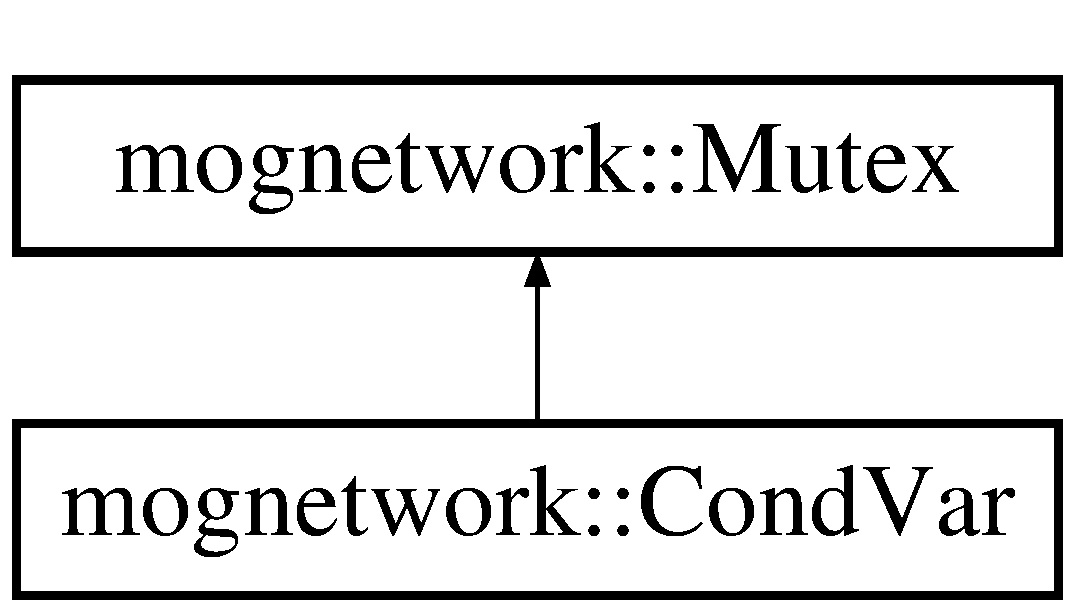
\includegraphics[height=2.000000cm]{classmognetwork_1_1_cond_var}
\end{center}
\end{figure}
\subsection*{Public Member Functions}
\begin{DoxyCompactItemize}
\item 
\hypertarget{classmognetwork_1_1_cond_var_ab7f3756ed998d61f8c4eec3d1f3a984b}{\hyperlink{classmognetwork_1_1_cond_var_ab7f3756ed998d61f8c4eec3d1f3a984b}{Cond\-Var} ()}\label{classmognetwork_1_1_cond_var_ab7f3756ed998d61f8c4eec3d1f3a984b}

\begin{DoxyCompactList}\small\item\em Constructeur par défaut. \end{DoxyCompactList}\item 
\hypertarget{classmognetwork_1_1_cond_var_afaee9fd061be682985bdc15d45e11816}{void \hyperlink{classmognetwork_1_1_cond_var_afaee9fd061be682985bdc15d45e11816}{wait} ()}\label{classmognetwork_1_1_cond_var_afaee9fd061be682985bdc15d45e11816}

\begin{DoxyCompactList}\small\item\em Attend que la cond\-Var soit notifiée. \end{DoxyCompactList}\item 
\hypertarget{classmognetwork_1_1_cond_var_aeb5e8e751376a09f36c115e342778d3f}{void \hyperlink{classmognetwork_1_1_cond_var_aeb5e8e751376a09f36c115e342778d3f}{signal} ()}\label{classmognetwork_1_1_cond_var_aeb5e8e751376a09f36c115e342778d3f}

\begin{DoxyCompactList}\small\item\em notifie la cond\-Var \end{DoxyCompactList}\item 
\hypertarget{classmognetwork_1_1_cond_var_ae407b095e176f8c360d1f03ceaac1ad7}{void \hyperlink{classmognetwork_1_1_cond_var_ae407b095e176f8c360d1f03ceaac1ad7}{broadcast} ()}\label{classmognetwork_1_1_cond_var_ae407b095e176f8c360d1f03ceaac1ad7}

\begin{DoxyCompactList}\small\item\em redémarre le thread de la cond\-Var \end{DoxyCompactList}\item 
\hypertarget{classmognetwork_1_1_cond_var_a75efe016cf3ea093555f302bd980ad34}{void {\bfseries timedwait} (const struct timespec $\ast$abstime)}\label{classmognetwork_1_1_cond_var_a75efe016cf3ea093555f302bd980ad34}

\end{DoxyCompactItemize}
\subsection*{Protected Attributes}
\begin{DoxyCompactItemize}
\item 
pthread\-\_\-cond\-\_\-t \hyperlink{classmognetwork_1_1_cond_var_adc18d17b3c2e11768b1103b499f49c97}{m\-\_\-cond}
\end{DoxyCompactItemize}


\subsection{Detailed Description}
Encapsulation des variables conditionnelles. 

\subsection{Member Data Documentation}
\hypertarget{classmognetwork_1_1_cond_var_adc18d17b3c2e11768b1103b499f49c97}{\index{mognetwork\-::\-Cond\-Var@{mognetwork\-::\-Cond\-Var}!m\-\_\-cond@{m\-\_\-cond}}
\index{m\-\_\-cond@{m\-\_\-cond}!mognetwork::CondVar@{mognetwork\-::\-Cond\-Var}}
\subsubsection[{m\-\_\-cond}]{\setlength{\rightskip}{0pt plus 5cm}pthread\-\_\-cond\-\_\-t mognetwork\-::\-Cond\-Var\-::m\-\_\-cond\hspace{0.3cm}{\ttfamily [protected]}}}\label{classmognetwork_1_1_cond_var_adc18d17b3c2e11768b1103b499f49c97}
Variable conditionnelle 

The documentation for this class was generated from the following file\-:\begin{DoxyCompactItemize}
\item 
include/\hyperlink{_cond_var_8hh}{Cond\-Var.\-hh}\end{DoxyCompactItemize}

\hypertarget{classmognetwork_1_1_ip_address}{\section{mognetwork\-:\-:Ip\-Address Class Reference}
\label{classmognetwork_1_1_ip_address}\index{mognetwork\-::\-Ip\-Address@{mognetwork\-::\-Ip\-Address}}
}


Permet la gestion d'addresses I\-P.  




{\ttfamily \#include $<$Ip\-Address.\-hh$>$}

\subsection*{Public Member Functions}
\begin{DoxyCompactItemize}
\item 
\hyperlink{classmognetwork_1_1_ip_address_ade946e9608a23cead8165d9600256458}{Ip\-Address} (const std\-::string \&address)
\begin{DoxyCompactList}\small\item\em Constructeur par défaut. \end{DoxyCompactList}\item 
int \hyperlink{classmognetwork_1_1_ip_address_a56ff31f84eb42a1c8a65a40fc67947d5}{get\-Int} () const 
\begin{DoxyCompactList}\small\item\em Renvoit la conversion en I\-N\-T de l'I\-P. \end{DoxyCompactList}\end{DoxyCompactItemize}


\subsection{Detailed Description}
Permet la gestion d'addresses I\-P. 

\subsection{Constructor \& Destructor Documentation}
\hypertarget{classmognetwork_1_1_ip_address_ade946e9608a23cead8165d9600256458}{\index{mognetwork\-::\-Ip\-Address@{mognetwork\-::\-Ip\-Address}!Ip\-Address@{Ip\-Address}}
\index{Ip\-Address@{Ip\-Address}!mognetwork::IpAddress@{mognetwork\-::\-Ip\-Address}}
\subsubsection[{Ip\-Address}]{\setlength{\rightskip}{0pt plus 5cm}mognetwork\-::\-Ip\-Address\-::\-Ip\-Address (
\begin{DoxyParamCaption}
\item[{const std\-::string \&}]{address}
\end{DoxyParamCaption}
)}}\label{classmognetwork_1_1_ip_address_ade946e9608a23cead8165d9600256458}


Constructeur par défaut. 


\begin{DoxyParams}{Parameters}
{\em address} & L'adresse à utiliser \\
\hline
\end{DoxyParams}


\subsection{Member Function Documentation}
\hypertarget{classmognetwork_1_1_ip_address_a56ff31f84eb42a1c8a65a40fc67947d5}{\index{mognetwork\-::\-Ip\-Address@{mognetwork\-::\-Ip\-Address}!get\-Int@{get\-Int}}
\index{get\-Int@{get\-Int}!mognetwork::IpAddress@{mognetwork\-::\-Ip\-Address}}
\subsubsection[{get\-Int}]{\setlength{\rightskip}{0pt plus 5cm}int mognetwork\-::\-Ip\-Address\-::get\-Int (
\begin{DoxyParamCaption}
{}
\end{DoxyParamCaption}
) const}}\label{classmognetwork_1_1_ip_address_a56ff31f84eb42a1c8a65a40fc67947d5}


Renvoit la conversion en I\-N\-T de l'I\-P. 

\begin{DoxyReturn}{Returns}
la conversion de l'ip en int 
\end{DoxyReturn}


The documentation for this class was generated from the following file\-:\begin{DoxyCompactItemize}
\item 
include/\hyperlink{_ip_address_8hh}{Ip\-Address.\-hh}\end{DoxyCompactItemize}

\hypertarget{classmognetwork_1_1_i_runnable}{\section{mognetwork\-:\-:I\-Runnable Class Reference}
\label{classmognetwork_1_1_i_runnable}\index{mognetwork\-::\-I\-Runnable@{mognetwork\-::\-I\-Runnable}}
}


Interface permettant de créer une fonction d'exécution pour les Threads (java style)  




{\ttfamily \#include $<$I\-Runnable.\-hh$>$}

\subsection*{Public Member Functions}
\begin{DoxyCompactItemize}
\item 
\hypertarget{classmognetwork_1_1_i_runnable_ac53515c8ecf2b2c79cb9c161fdd600d1}{virtual void \hyperlink{classmognetwork_1_1_i_runnable_ac53515c8ecf2b2c79cb9c161fdd600d1}{run} ()=0}\label{classmognetwork_1_1_i_runnable_ac53515c8ecf2b2c79cb9c161fdd600d1}

\begin{DoxyCompactList}\small\item\em fonction utilisée par les threads en temps que pointeur sur fonction \end{DoxyCompactList}\end{DoxyCompactItemize}


\subsection{Detailed Description}
Interface permettant de créer une fonction d'exécution pour les Threads (java style) 

The documentation for this class was generated from the following file\-:\begin{DoxyCompactItemize}
\item 
include/\hyperlink{_i_runnable_8hh}{I\-Runnable.\-hh}\end{DoxyCompactItemize}

\hypertarget{classmognetwork_1_1_i_tcp_a_s_i_o_listener_handler}{\section{mognetwork\-:\-:I\-Tcp\-A\-S\-I\-O\-Listener\-Handler Class Reference}
\label{classmognetwork_1_1_i_tcp_a_s_i_o_listener_handler}\index{mognetwork\-::\-I\-Tcp\-A\-S\-I\-O\-Listener\-Handler@{mognetwork\-::\-I\-Tcp\-A\-S\-I\-O\-Listener\-Handler}}
}
\subsection*{Public Member Functions}
\begin{DoxyCompactItemize}
\item 
virtual void \hyperlink{classmognetwork_1_1_i_tcp_a_s_i_o_listener_handler_aa1d6b507fc5adc689698c6bd7f0a8ca0}{on\-Connect} (\hyperlink{classmognetwork_1_1_tcp_socket}{Tcp\-Socket} \&client)=0
\begin{DoxyCompactList}\small\item\em Appelé lors de la connexion d'un nouveau client. \end{DoxyCompactList}\item 
virtual void \hyperlink{classmognetwork_1_1_i_tcp_a_s_i_o_listener_handler_a8cc4a40b4addfc1abdf94ba66a545674}{on\-Received\-Data} (\hyperlink{classmognetwork_1_1_tcp_socket}{Tcp\-Socket} \&client)=0
\begin{DoxyCompactList}\small\item\em Appelé lors de la réception totale d'une donnée. \end{DoxyCompactList}\item 
virtual void \hyperlink{classmognetwork_1_1_i_tcp_a_s_i_o_listener_handler_afeb615cb2f1e1f543a6282e21e66c543}{on\-Disconnect} (\hyperlink{classmognetwork_1_1_tcp_socket}{Tcp\-Socket} \&client)=0
\begin{DoxyCompactList}\small\item\em Appelé lors de la déconnexion d'un client. \end{DoxyCompactList}\end{DoxyCompactItemize}


\subsection{Member Function Documentation}
\hypertarget{classmognetwork_1_1_i_tcp_a_s_i_o_listener_handler_aa1d6b507fc5adc689698c6bd7f0a8ca0}{\index{mognetwork\-::\-I\-Tcp\-A\-S\-I\-O\-Listener\-Handler@{mognetwork\-::\-I\-Tcp\-A\-S\-I\-O\-Listener\-Handler}!on\-Connect@{on\-Connect}}
\index{on\-Connect@{on\-Connect}!mognetwork::ITcpASIOListenerHandler@{mognetwork\-::\-I\-Tcp\-A\-S\-I\-O\-Listener\-Handler}}
\subsubsection[{on\-Connect}]{\setlength{\rightskip}{0pt plus 5cm}virtual void mognetwork\-::\-I\-Tcp\-A\-S\-I\-O\-Listener\-Handler\-::on\-Connect (
\begin{DoxyParamCaption}
\item[{{\bf Tcp\-Socket} \&}]{client}
\end{DoxyParamCaption}
)\hspace{0.3cm}{\ttfamily [pure virtual]}}}\label{classmognetwork_1_1_i_tcp_a_s_i_o_listener_handler_aa1d6b507fc5adc689698c6bd7f0a8ca0}


Appelé lors de la connexion d'un nouveau client. 


\begin{DoxyParams}{Parameters}
{\em client} & le client qui c'est connecté \\
\hline
\end{DoxyParams}
\hypertarget{classmognetwork_1_1_i_tcp_a_s_i_o_listener_handler_afeb615cb2f1e1f543a6282e21e66c543}{\index{mognetwork\-::\-I\-Tcp\-A\-S\-I\-O\-Listener\-Handler@{mognetwork\-::\-I\-Tcp\-A\-S\-I\-O\-Listener\-Handler}!on\-Disconnect@{on\-Disconnect}}
\index{on\-Disconnect@{on\-Disconnect}!mognetwork::ITcpASIOListenerHandler@{mognetwork\-::\-I\-Tcp\-A\-S\-I\-O\-Listener\-Handler}}
\subsubsection[{on\-Disconnect}]{\setlength{\rightskip}{0pt plus 5cm}virtual void mognetwork\-::\-I\-Tcp\-A\-S\-I\-O\-Listener\-Handler\-::on\-Disconnect (
\begin{DoxyParamCaption}
\item[{{\bf Tcp\-Socket} \&}]{client}
\end{DoxyParamCaption}
)\hspace{0.3cm}{\ttfamily [pure virtual]}}}\label{classmognetwork_1_1_i_tcp_a_s_i_o_listener_handler_afeb615cb2f1e1f543a6282e21e66c543}


Appelé lors de la déconnexion d'un client. 


\begin{DoxyParams}{Parameters}
{\em client} & le client qui c'est déconnecté \\
\hline
\end{DoxyParams}
\hypertarget{classmognetwork_1_1_i_tcp_a_s_i_o_listener_handler_a8cc4a40b4addfc1abdf94ba66a545674}{\index{mognetwork\-::\-I\-Tcp\-A\-S\-I\-O\-Listener\-Handler@{mognetwork\-::\-I\-Tcp\-A\-S\-I\-O\-Listener\-Handler}!on\-Received\-Data@{on\-Received\-Data}}
\index{on\-Received\-Data@{on\-Received\-Data}!mognetwork::ITcpASIOListenerHandler@{mognetwork\-::\-I\-Tcp\-A\-S\-I\-O\-Listener\-Handler}}
\subsubsection[{on\-Received\-Data}]{\setlength{\rightskip}{0pt plus 5cm}virtual void mognetwork\-::\-I\-Tcp\-A\-S\-I\-O\-Listener\-Handler\-::on\-Received\-Data (
\begin{DoxyParamCaption}
\item[{{\bf Tcp\-Socket} \&}]{client}
\end{DoxyParamCaption}
)\hspace{0.3cm}{\ttfamily [pure virtual]}}}\label{classmognetwork_1_1_i_tcp_a_s_i_o_listener_handler_a8cc4a40b4addfc1abdf94ba66a545674}


Appelé lors de la réception totale d'une donnée. 


\begin{DoxyParams}{Parameters}
{\em client} & le client qui a trigger les données \\
\hline
\end{DoxyParams}


The documentation for this class was generated from the following file\-:\begin{DoxyCompactItemize}
\item 
include/mognetwork/\hyperlink{_i_tcp_a_s_i_o_listener_handler_8hh}{I\-Tcp\-A\-S\-I\-O\-Listener\-Handler.\-hh}\end{DoxyCompactItemize}

\hypertarget{class_i_tcp_a_s_i_o_listerner_handler}{\section{I\-Tcp\-A\-S\-I\-O\-Listerner\-Handler Class Reference}
\label{class_i_tcp_a_s_i_o_listerner_handler}\index{I\-Tcp\-A\-S\-I\-O\-Listerner\-Handler@{I\-Tcp\-A\-S\-I\-O\-Listerner\-Handler}}
}


Handler pour le Tcp\-A\-S\-I\-O\-Listener.  




{\ttfamily \#include $<$I\-Tcp\-A\-S\-I\-O\-Listener\-Handler.\-hh$>$}



\subsection{Detailed Description}
Handler pour le Tcp\-A\-S\-I\-O\-Listener. 

The documentation for this class was generated from the following file\-:\begin{DoxyCompactItemize}
\item 
include/\hyperlink{_i_tcp_a_s_i_o_listener_handler_8hh}{I\-Tcp\-A\-S\-I\-O\-Listener\-Handler.\-hh}\end{DoxyCompactItemize}

\hypertarget{classmognetwork_1_1_lib_network_exception}{\section{mognetwork\-:\-:Lib\-Network\-Exception Class Reference}
\label{classmognetwork_1_1_lib_network_exception}\index{mognetwork\-::\-Lib\-Network\-Exception@{mognetwork\-::\-Lib\-Network\-Exception}}
}


Lib\-Net exceptions.  




{\ttfamily \#include $<$Lib\-Network\-Exception.\-hh$>$}

Inheritance diagram for mognetwork\-:\-:Lib\-Network\-Exception\-:\begin{figure}[H]
\begin{center}
\leavevmode
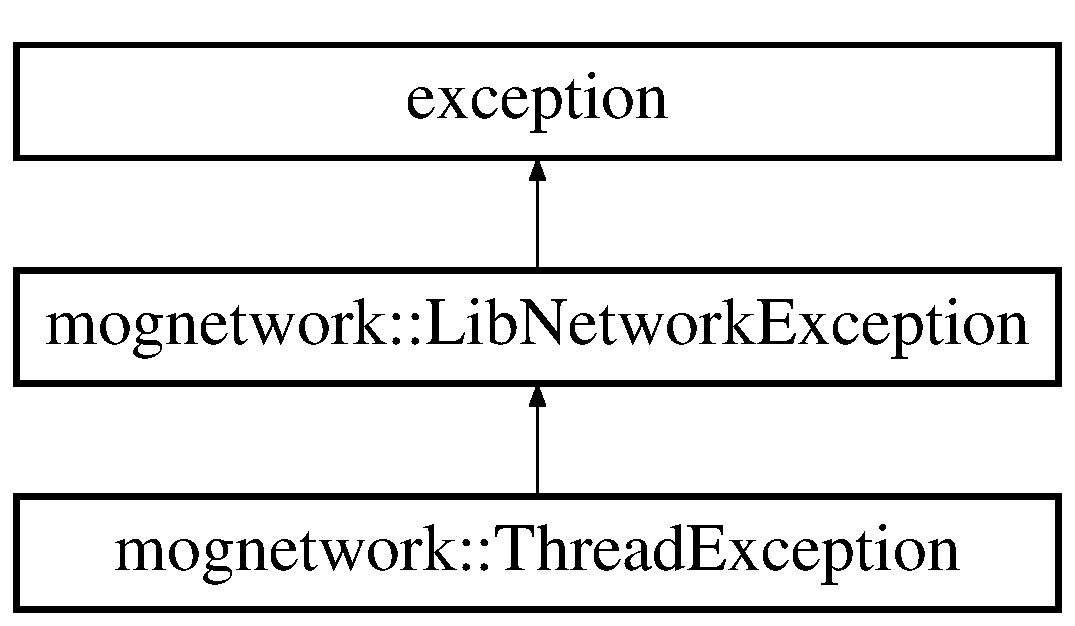
\includegraphics[height=3.000000cm]{classmognetwork_1_1_lib_network_exception}
\end{center}
\end{figure}
\subsection*{Public Member Functions}
\begin{DoxyCompactItemize}
\item 
\hyperlink{classmognetwork_1_1_lib_network_exception_af74972d2d7160710b8faaccb01f6455c}{Lib\-Network\-Exception} (const char $\ast$msg, int line, const char $\ast$file)
\begin{DoxyCompactList}\small\item\em Default constructor. \end{DoxyCompactList}\item 
virtual const char $\ast$ \hyperlink{classmognetwork_1_1_lib_network_exception_a65c5c92d2bf25a9c4cd8a0322c36e54a}{what} () const   throw ()
\begin{DoxyCompactList}\small\item\em Get the error message. \end{DoxyCompactList}\end{DoxyCompactItemize}


\subsection{Detailed Description}
Lib\-Net exceptions. 

\subsection{Constructor \& Destructor Documentation}
\hypertarget{classmognetwork_1_1_lib_network_exception_af74972d2d7160710b8faaccb01f6455c}{\index{mognetwork\-::\-Lib\-Network\-Exception@{mognetwork\-::\-Lib\-Network\-Exception}!Lib\-Network\-Exception@{Lib\-Network\-Exception}}
\index{Lib\-Network\-Exception@{Lib\-Network\-Exception}!mognetwork::LibNetworkException@{mognetwork\-::\-Lib\-Network\-Exception}}
\subsubsection[{Lib\-Network\-Exception}]{\setlength{\rightskip}{0pt plus 5cm}mognetwork\-::\-Lib\-Network\-Exception\-::\-Lib\-Network\-Exception (
\begin{DoxyParamCaption}
\item[{const char $\ast$}]{msg, }
\item[{int}]{line, }
\item[{const char $\ast$}]{file}
\end{DoxyParamCaption}
)\hspace{0.3cm}{\ttfamily [inline]}}}\label{classmognetwork_1_1_lib_network_exception_af74972d2d7160710b8faaccb01f6455c}


Default constructor. 


\begin{DoxyParams}{Parameters}
{\em msg} & Error message \\
\hline
{\em line} & Line of the error. Usually {\bfseries L\-I\-N\-E} \\
\hline
{\em file} & File of the error. Usually {\bfseries F\-I\-L\-E} \\
\hline
\end{DoxyParams}


\subsection{Member Function Documentation}
\hypertarget{classmognetwork_1_1_lib_network_exception_a65c5c92d2bf25a9c4cd8a0322c36e54a}{\index{mognetwork\-::\-Lib\-Network\-Exception@{mognetwork\-::\-Lib\-Network\-Exception}!what@{what}}
\index{what@{what}!mognetwork::LibNetworkException@{mognetwork\-::\-Lib\-Network\-Exception}}
\subsubsection[{what}]{\setlength{\rightskip}{0pt plus 5cm}virtual const char$\ast$ mognetwork\-::\-Lib\-Network\-Exception\-::what (
\begin{DoxyParamCaption}
{}
\end{DoxyParamCaption}
) const throw  ) \hspace{0.3cm}{\ttfamily [inline]}, {\ttfamily [virtual]}}}\label{classmognetwork_1_1_lib_network_exception_a65c5c92d2bf25a9c4cd8a0322c36e54a}


Get the error message. 

\begin{DoxyReturn}{Returns}
The error message 
\end{DoxyReturn}


The documentation for this class was generated from the following file\-:\begin{DoxyCompactItemize}
\item 
include/mognetwork/\hyperlink{_lib_network_exception_8hh}{Lib\-Network\-Exception.\-hh}\end{DoxyCompactItemize}

\hypertarget{classmognetwork_1_1_mutex}{\section{mognetwork\-:\-:Mutex Class Reference}
\label{classmognetwork_1_1_mutex}\index{mognetwork\-::\-Mutex@{mognetwork\-::\-Mutex}}
}


Encapsulation des \hyperlink{classmognetwork_1_1_mutex}{Mutex}.  




{\ttfamily \#include $<$Mutex.\-hh$>$}

Inheritance diagram for mognetwork\-:\-:Mutex\-:\begin{figure}[H]
\begin{center}
\leavevmode
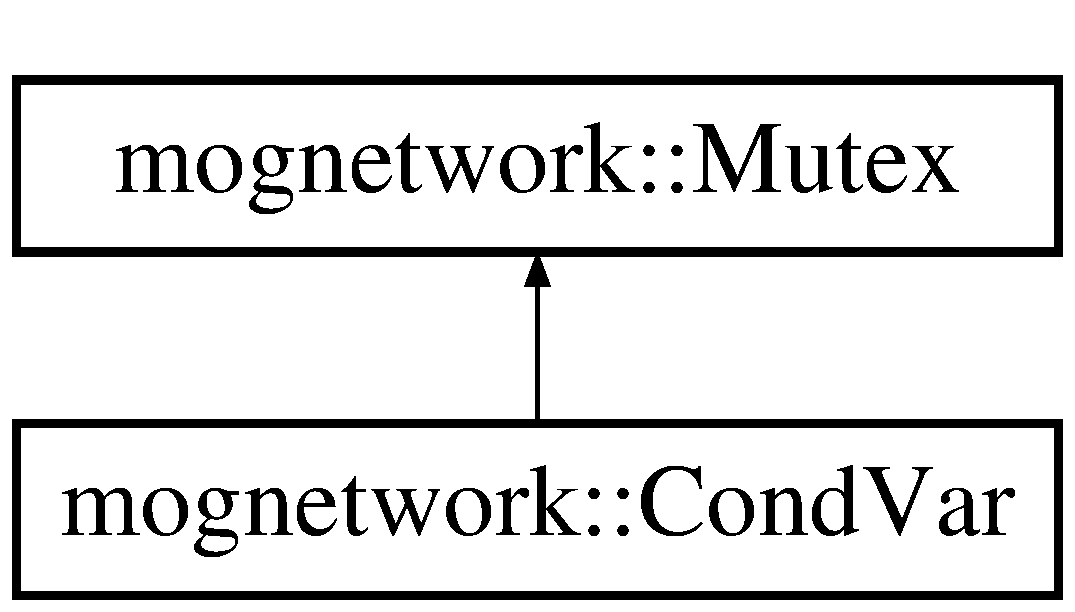
\includegraphics[height=2.000000cm]{classmognetwork_1_1_mutex}
\end{center}
\end{figure}
\subsection*{Public Member Functions}
\begin{DoxyCompactItemize}
\item 
\hypertarget{classmognetwork_1_1_mutex_a281ab0e408b9a388586ee269881d3c26}{\hyperlink{classmognetwork_1_1_mutex_a281ab0e408b9a388586ee269881d3c26}{Mutex} ()}\label{classmognetwork_1_1_mutex_a281ab0e408b9a388586ee269881d3c26}

\begin{DoxyCompactList}\small\item\em Constructeur par défaut. \end{DoxyCompactList}\item 
\hypertarget{classmognetwork_1_1_mutex_a880c4341ad8d63c9bde15f4a60af2848}{void \hyperlink{classmognetwork_1_1_mutex_a880c4341ad8d63c9bde15f4a60af2848}{lock} ()}\label{classmognetwork_1_1_mutex_a880c4341ad8d63c9bde15f4a60af2848}

\begin{DoxyCompactList}\small\item\em block un mutex \end{DoxyCompactList}\item 
\hypertarget{classmognetwork_1_1_mutex_a9f3e0b542f8e9953eca9df6ae408083e}{void \hyperlink{classmognetwork_1_1_mutex_a9f3e0b542f8e9953eca9df6ae408083e}{unlock} ()}\label{classmognetwork_1_1_mutex_a9f3e0b542f8e9953eca9df6ae408083e}

\begin{DoxyCompactList}\small\item\em délock un mutex \end{DoxyCompactList}\item 
\hypertarget{classmognetwork_1_1_mutex_a80d976553316b396cb74cc335fcca31a}{void \hyperlink{classmognetwork_1_1_mutex_a80d976553316b396cb74cc335fcca31a}{trylock} ()}\label{classmognetwork_1_1_mutex_a80d976553316b396cb74cc335fcca31a}

\begin{DoxyCompactList}\small\item\em trylock un mutex \end{DoxyCompactList}\end{DoxyCompactItemize}
\subsection*{Protected Attributes}
\begin{DoxyCompactItemize}
\item 
pthread\-\_\-mutex\-\_\-t \hyperlink{classmognetwork_1_1_mutex_a571d9d0b9b2be3da94192f34b6157ea9}{m\-\_\-mutex}
\end{DoxyCompactItemize}


\subsection{Detailed Description}
Encapsulation des \hyperlink{classmognetwork_1_1_mutex}{Mutex}. 

\subsection{Member Data Documentation}
\hypertarget{classmognetwork_1_1_mutex_a571d9d0b9b2be3da94192f34b6157ea9}{\index{mognetwork\-::\-Mutex@{mognetwork\-::\-Mutex}!m\-\_\-mutex@{m\-\_\-mutex}}
\index{m\-\_\-mutex@{m\-\_\-mutex}!mognetwork::Mutex@{mognetwork\-::\-Mutex}}
\subsubsection[{m\-\_\-mutex}]{\setlength{\rightskip}{0pt plus 5cm}pthread\-\_\-mutex\-\_\-t mognetwork\-::\-Mutex\-::m\-\_\-mutex\hspace{0.3cm}{\ttfamily [protected]}}}\label{classmognetwork_1_1_mutex_a571d9d0b9b2be3da94192f34b6157ea9}
données de la mutex 

The documentation for this class was generated from the following file\-:\begin{DoxyCompactItemize}
\item 
include/\hyperlink{_mutex_8hh}{Mutex.\-hh}\end{DoxyCompactItemize}

\hypertarget{classmognetwork_1_1_os_socket}{\section{mognetwork\-:\-:Os\-Socket Class Reference}
\label{classmognetwork_1_1_os_socket}\index{mognetwork\-::\-Os\-Socket@{mognetwork\-::\-Os\-Socket}}
}


Implementation of the windows sockets.  




{\ttfamily \#include $<$Win\-Socket.\-hh$>$}

\subsection*{Public Types}
\begin{DoxyCompactItemize}
\item 
\hypertarget{classmognetwork_1_1_os_socket_a10e453b27c0954f12f5dbf74bf9853c0}{typedef socklen\-\_\-t {\bfseries Addr\-Length}}\label{classmognetwork_1_1_os_socket_a10e453b27c0954f12f5dbf74bf9853c0}

\item 
typedef int \hyperlink{classmognetwork_1_1_os_socket_a53fd4fa9dc6b02cafdb4b7a2b6d94778}{Addre\-Length}
\end{DoxyCompactItemize}
\subsection*{Static Public Member Functions}
\begin{DoxyCompactItemize}
\item 
\hypertarget{classmognetwork_1_1_os_socket_aec3ee68397d04abab9003ddd68e86793}{static sockaddr\-\_\-in {\bfseries create\-Address} (uint32\-\_\-t address, unsigned short port)}\label{classmognetwork_1_1_os_socket_aec3ee68397d04abab9003ddd68e86793}

\item 
\hypertarget{classmognetwork_1_1_os_socket_a5b2cf6583d7bc3a640a162a6ae3dead7}{static Socket\-F\-D {\bfseries not\-Valid} ()}\label{classmognetwork_1_1_os_socket_a5b2cf6583d7bc3a640a162a6ae3dead7}

\item 
\hypertarget{classmognetwork_1_1_os_socket_afc41f453da34be5cce9fa5470ca3697a}{static void {\bfseries close} (Socket\-F\-D socket)}\label{classmognetwork_1_1_os_socket_afc41f453da34be5cce9fa5470ca3697a}

\item 
\hypertarget{classmognetwork_1_1_os_socket_a331f63335ee89ae3eaa24a59cbada192}{static \hyperlink{classmognetwork_1_1_socket_aa187a8394ac0d6203af0ec7f021ca15f}{Socket\-::\-Status} {\bfseries get\-Error\-Status} ()}\label{classmognetwork_1_1_os_socket_a331f63335ee89ae3eaa24a59cbada192}

\item 
static sockaddr\-\_\-in \hyperlink{classmognetwork_1_1_os_socket_ae012b09d94070d07925a03cdc3a8a6ae}{create\-Address} (Uint32 address, unsigned short port)
\begin{DoxyCompactList}\small\item\em create a sockaddr\-\_\-in \end{DoxyCompactList}\item 
static Socket\-F\-D \hyperlink{classmognetwork_1_1_os_socket_a5b2cf6583d7bc3a640a162a6ae3dead7}{not\-Valid} ()
\begin{DoxyCompactList}\small\item\em Get the socket state of an unvalid socket. \end{DoxyCompactList}\item 
static void \hyperlink{classmognetwork_1_1_os_socket_afc41f453da34be5cce9fa5470ca3697a}{close} (Socket\-F\-D socket)
\begin{DoxyCompactList}\small\item\em Close the socket. \end{DoxyCompactList}\item 
static \hyperlink{classmognetwork_1_1_socket_aa187a8394ac0d6203af0ec7f021ca15f}{Socket\-::\-Status} \hyperlink{classmognetwork_1_1_os_socket_a331f63335ee89ae3eaa24a59cbada192}{get\-Error\-Status} ()
\begin{DoxyCompactList}\small\item\em Get the error status of the socket. \end{DoxyCompactList}\end{DoxyCompactItemize}


\subsection{Detailed Description}
Implementation of the windows sockets. 

\subsection{Member Typedef Documentation}
\hypertarget{classmognetwork_1_1_os_socket_a53fd4fa9dc6b02cafdb4b7a2b6d94778}{\index{mognetwork\-::\-Os\-Socket@{mognetwork\-::\-Os\-Socket}!Addre\-Length@{Addre\-Length}}
\index{Addre\-Length@{Addre\-Length}!mognetwork::OsSocket@{mognetwork\-::\-Os\-Socket}}
\subsubsection[{Addre\-Length}]{\setlength{\rightskip}{0pt plus 5cm}typedef int {\bf mognetwork\-::\-Os\-Socket\-::\-Addre\-Length}}}\label{classmognetwork_1_1_os_socket_a53fd4fa9dc6b02cafdb4b7a2b6d94778}
length of an address 

\subsection{Member Function Documentation}
\hypertarget{classmognetwork_1_1_os_socket_afc41f453da34be5cce9fa5470ca3697a}{\index{mognetwork\-::\-Os\-Socket@{mognetwork\-::\-Os\-Socket}!close@{close}}
\index{close@{close}!mognetwork::OsSocket@{mognetwork\-::\-Os\-Socket}}
\subsubsection[{close}]{\setlength{\rightskip}{0pt plus 5cm}static void mognetwork\-::\-Os\-Socket\-::close (
\begin{DoxyParamCaption}
\item[{Socket\-F\-D}]{socket}
\end{DoxyParamCaption}
)\hspace{0.3cm}{\ttfamily [static]}}}\label{classmognetwork_1_1_os_socket_afc41f453da34be5cce9fa5470ca3697a}


Close the socket. 


\begin{DoxyParams}{Parameters}
{\em socket} & the Socket\-F\-D to close \\
\hline
\end{DoxyParams}
\hypertarget{classmognetwork_1_1_os_socket_ae012b09d94070d07925a03cdc3a8a6ae}{\index{mognetwork\-::\-Os\-Socket@{mognetwork\-::\-Os\-Socket}!create\-Address@{create\-Address}}
\index{create\-Address@{create\-Address}!mognetwork::OsSocket@{mognetwork\-::\-Os\-Socket}}
\subsubsection[{create\-Address}]{\setlength{\rightskip}{0pt plus 5cm}static sockaddr\-\_\-in mognetwork\-::\-Os\-Socket\-::create\-Address (
\begin{DoxyParamCaption}
\item[{Uint32}]{address, }
\item[{unsigned short}]{port}
\end{DoxyParamCaption}
)\hspace{0.3cm}{\ttfamily [static]}}}\label{classmognetwork_1_1_os_socket_ae012b09d94070d07925a03cdc3a8a6ae}


create a sockaddr\-\_\-in 


\begin{DoxyParams}{Parameters}
{\em address} & \-: the address in Uint32 \\
\hline
{\em port} & \-: the port to use \\
\hline
\end{DoxyParams}
\begin{DoxyReturn}{Returns}
sockaddr\-\_\-in the initialised structure 
\end{DoxyReturn}
\hypertarget{classmognetwork_1_1_os_socket_a331f63335ee89ae3eaa24a59cbada192}{\index{mognetwork\-::\-Os\-Socket@{mognetwork\-::\-Os\-Socket}!get\-Error\-Status@{get\-Error\-Status}}
\index{get\-Error\-Status@{get\-Error\-Status}!mognetwork::OsSocket@{mognetwork\-::\-Os\-Socket}}
\subsubsection[{get\-Error\-Status}]{\setlength{\rightskip}{0pt plus 5cm}static {\bf Socket\-::\-Status} mognetwork\-::\-Os\-Socket\-::get\-Error\-Status (
\begin{DoxyParamCaption}
{}
\end{DoxyParamCaption}
)\hspace{0.3cm}{\ttfamily [static]}}}\label{classmognetwork_1_1_os_socket_a331f63335ee89ae3eaa24a59cbada192}


Get the error status of the socket. 

\begin{DoxyReturn}{Returns}
\hyperlink{classmognetwork_1_1_socket_aa187a8394ac0d6203af0ec7f021ca15f}{Socket\-::\-Status} the status of the socket 
\end{DoxyReturn}
\hypertarget{classmognetwork_1_1_os_socket_a5b2cf6583d7bc3a640a162a6ae3dead7}{\index{mognetwork\-::\-Os\-Socket@{mognetwork\-::\-Os\-Socket}!not\-Valid@{not\-Valid}}
\index{not\-Valid@{not\-Valid}!mognetwork::OsSocket@{mognetwork\-::\-Os\-Socket}}
\subsubsection[{not\-Valid}]{\setlength{\rightskip}{0pt plus 5cm}static Socket\-F\-D mognetwork\-::\-Os\-Socket\-::not\-Valid (
\begin{DoxyParamCaption}
{}
\end{DoxyParamCaption}
)\hspace{0.3cm}{\ttfamily [static]}}}\label{classmognetwork_1_1_os_socket_a5b2cf6583d7bc3a640a162a6ae3dead7}


Get the socket state of an unvalid socket. 

\begin{DoxyReturn}{Returns}
Socket\-F\-D a unvalid fd 
\end{DoxyReturn}


The documentation for this class was generated from the following files\-:\begin{DoxyCompactItemize}
\item 
include/mognetwork/Unix\-Socket.\-hh\item 
include/mognetwork/\hyperlink{_win_socket_8hh}{Win\-Socket.\-hh}\end{DoxyCompactItemize}

\hypertarget{structmognetwork_1_1_tcp_socket_1_1_readed_datas}{\section{mognetwork\-:\-:Tcp\-Socket\-:\-:Readed\-Datas Struct Reference}
\label{structmognetwork_1_1_tcp_socket_1_1_readed_datas}\index{mognetwork\-::\-Tcp\-Socket\-::\-Readed\-Datas@{mognetwork\-::\-Tcp\-Socket\-::\-Readed\-Datas}}
}


Has all the datas to retrive and send process in A\-S\-I\-O.  




{\ttfamily \#include $<$Tcp\-Socket.\-hh$>$}

\subsection*{Public Member Functions}
\begin{DoxyCompactItemize}
\item 
\hyperlink{structmognetwork_1_1_tcp_socket_1_1_readed_datas_a5f000677cc0bfc88c3ab563ede5907ab}{Readed\-Datas} ()
\end{DoxyCompactItemize}
\subsection*{Public Attributes}
\begin{DoxyCompactItemize}
\item 
std\-::size\-\_\-t \hyperlink{structmognetwork_1_1_tcp_socket_1_1_readed_datas_a2c633a79efa956f1f59d9429e8584cc0}{readed}
\item 
std\-::size\-\_\-t \hyperlink{structmognetwork_1_1_tcp_socket_1_1_readed_datas_aac0aa498d4b98296434cf05785068dcc}{total\-Size}
\item 
\hyperlink{classmognetwork_1_1_tcp_socket_aa80d910649a16cedb6c98297e5893ed1}{Data} \hyperlink{structmognetwork_1_1_tcp_socket_1_1_readed_datas_abfdc3750f4970fde4212d7a0e934daa9}{datas}
\end{DoxyCompactItemize}


\subsection{Detailed Description}
Has all the datas to retrive and send process in A\-S\-I\-O. 

\subsection{Constructor \& Destructor Documentation}
\hypertarget{structmognetwork_1_1_tcp_socket_1_1_readed_datas_a5f000677cc0bfc88c3ab563ede5907ab}{\index{mognetwork\-::\-Tcp\-Socket\-::\-Readed\-Datas@{mognetwork\-::\-Tcp\-Socket\-::\-Readed\-Datas}!Readed\-Datas@{Readed\-Datas}}
\index{Readed\-Datas@{Readed\-Datas}!mognetwork::TcpSocket::ReadedDatas@{mognetwork\-::\-Tcp\-Socket\-::\-Readed\-Datas}}
\subsubsection[{Readed\-Datas}]{\setlength{\rightskip}{0pt plus 5cm}mognetwork\-::\-Tcp\-Socket\-::\-Readed\-Datas\-::\-Readed\-Datas (
\begin{DoxyParamCaption}
{}
\end{DoxyParamCaption}
)}}\label{structmognetwork_1_1_tcp_socket_1_1_readed_datas_a5f000677cc0bfc88c3ab563ede5907ab}
Used to init the structure 

\subsection{Member Data Documentation}
\hypertarget{structmognetwork_1_1_tcp_socket_1_1_readed_datas_abfdc3750f4970fde4212d7a0e934daa9}{\index{mognetwork\-::\-Tcp\-Socket\-::\-Readed\-Datas@{mognetwork\-::\-Tcp\-Socket\-::\-Readed\-Datas}!datas@{datas}}
\index{datas@{datas}!mognetwork::TcpSocket::ReadedDatas@{mognetwork\-::\-Tcp\-Socket\-::\-Readed\-Datas}}
\subsubsection[{datas}]{\setlength{\rightskip}{0pt plus 5cm}{\bf Data} mognetwork\-::\-Tcp\-Socket\-::\-Readed\-Datas\-::datas}}\label{structmognetwork_1_1_tcp_socket_1_1_readed_datas_abfdc3750f4970fde4212d7a0e934daa9}
Readed datas \hypertarget{structmognetwork_1_1_tcp_socket_1_1_readed_datas_a2c633a79efa956f1f59d9429e8584cc0}{\index{mognetwork\-::\-Tcp\-Socket\-::\-Readed\-Datas@{mognetwork\-::\-Tcp\-Socket\-::\-Readed\-Datas}!readed@{readed}}
\index{readed@{readed}!mognetwork::TcpSocket::ReadedDatas@{mognetwork\-::\-Tcp\-Socket\-::\-Readed\-Datas}}
\subsubsection[{readed}]{\setlength{\rightskip}{0pt plus 5cm}std\-::size\-\_\-t mognetwork\-::\-Tcp\-Socket\-::\-Readed\-Datas\-::readed}}\label{structmognetwork_1_1_tcp_socket_1_1_readed_datas_a2c633a79efa956f1f59d9429e8584cc0}
Bytes readed \hypertarget{structmognetwork_1_1_tcp_socket_1_1_readed_datas_aac0aa498d4b98296434cf05785068dcc}{\index{mognetwork\-::\-Tcp\-Socket\-::\-Readed\-Datas@{mognetwork\-::\-Tcp\-Socket\-::\-Readed\-Datas}!total\-Size@{total\-Size}}
\index{total\-Size@{total\-Size}!mognetwork::TcpSocket::ReadedDatas@{mognetwork\-::\-Tcp\-Socket\-::\-Readed\-Datas}}
\subsubsection[{total\-Size}]{\setlength{\rightskip}{0pt plus 5cm}std\-::size\-\_\-t mognetwork\-::\-Tcp\-Socket\-::\-Readed\-Datas\-::total\-Size}}\label{structmognetwork_1_1_tcp_socket_1_1_readed_datas_aac0aa498d4b98296434cf05785068dcc}
Total size to read 

The documentation for this struct was generated from the following file\-:\begin{DoxyCompactItemize}
\item 
include/mognetwork/\hyperlink{_tcp_socket_8hh}{Tcp\-Socket.\-hh}\end{DoxyCompactItemize}

\hypertarget{classmognetwork_1_1_selector}{\section{mognetwork\-:\-:Selector Class Reference}
\label{classmognetwork_1_1_selector}\index{mognetwork\-::\-Selector@{mognetwork\-::\-Selector}}
}


Select encapsulation.  




{\ttfamily \#include $<$Selector.\-hh$>$}

\subsection*{Public Types}
\begin{DoxyCompactItemize}
\item 
enum \hyperlink{classmognetwork_1_1_selector_a51d709c3579bf32265d68d4313df5794}{State} \{ {\bfseries Waiting}, 
{\bfseries Error}
 \}
\begin{DoxyCompactList}\small\item\em Defines the states of the select. \end{DoxyCompactList}\end{DoxyCompactItemize}
\subsection*{Public Member Functions}
\begin{DoxyCompactItemize}
\item 
\hypertarget{classmognetwork_1_1_selector_ac2dc59256b3b676a6c04102f5ea5515a}{\hyperlink{classmognetwork_1_1_selector_ac2dc59256b3b676a6c04102f5ea5515a}{Selector} ()}\label{classmognetwork_1_1_selector_ac2dc59256b3b676a6c04102f5ea5515a}

\begin{DoxyCompactList}\small\item\em Default constructor. \end{DoxyCompactList}\item 
\hypertarget{classmognetwork_1_1_selector_aba14d0165c8b6408e75a8a7db3cbffb7}{void \hyperlink{classmognetwork_1_1_selector_aba14d0165c8b6408e75a8a7db3cbffb7}{wait\-For\-Trigger} ()}\label{classmognetwork_1_1_selector_aba14d0165c8b6408e75a8a7db3cbffb7}

\begin{DoxyCompactList}\small\item\em Wait for a new update of the \hyperlink{classmognetwork_1_1_selector}{Selector}. \end{DoxyCompactList}\item 
\hyperlink{_selector_8hh_af47ac292ef7224cf549b944d138ba4ae}{Time} $\ast$ \hyperlink{classmognetwork_1_1_selector_ae1cb38fe53e4313751062277b39fbfd5}{get\-Timeout} () const 
\begin{DoxyCompactList}\small\item\em Get the timeout value. \end{DoxyCompactList}\item 
\hyperlink{classmognetwork_1_1_selector_a51d709c3579bf32265d68d4313df5794}{State} \hyperlink{classmognetwork_1_1_selector_aab8261de074ef927dfe62bb9ddaafb93}{get\-State} () const 
\begin{DoxyCompactList}\small\item\em Get the actual state of the \hyperlink{classmognetwork_1_1_selector}{Selector}. \end{DoxyCompactList}\item 
\hypertarget{classmognetwork_1_1_selector_ab35641925422b2082de069f745e0034e}{const std\-::list$<$ Socket\-F\-D $>$ \& \hyperlink{classmognetwork_1_1_selector_ab35641925422b2082de069f745e0034e}{get\-Writing\-Triggered\-Sockets} () const }\label{classmognetwork_1_1_selector_ab35641925422b2082de069f745e0034e}

\begin{DoxyCompactList}\small\item\em Get the socket list that are ready to be edited in writing mode  The list of the Socket\-F\-D. \end{DoxyCompactList}\item 
const std\-::list$<$ Socket\-F\-D $>$ \& \hyperlink{classmognetwork_1_1_selector_ae41a4ff4e9281cdd03880f69c0c71a35}{get\-Reading\-Triggered\-Sockets} () const 
\begin{DoxyCompactList}\small\item\em Get the socket list that are ready to be readed. \end{DoxyCompactList}\item 
void \hyperlink{classmognetwork_1_1_selector_ac03b53749206d8ba80dec22bad55e0a8}{set\-Timeout} (\hyperlink{_selector_8hh_af47ac292ef7224cf549b944d138ba4ae}{Time} $\ast$timeout)
\begin{DoxyCompactList}\small\item\em Defines a value for the timeout. \end{DoxyCompactList}\item 
void \hyperlink{classmognetwork_1_1_selector_a6f22d28dc38b5d252c0590de857d67f7}{add\-Fd\-To\-Write} (Socket\-F\-D fd)
\begin{DoxyCompactList}\small\item\em Add a fd to the writing trigger. \end{DoxyCompactList}\item 
void \hyperlink{classmognetwork_1_1_selector_aacc48e5256e3b5150f80acad84b82de3}{add\-Fd\-To\-Read} (Socket\-F\-D fd)
\begin{DoxyCompactList}\small\item\em Add a fd to the reading trigger. \end{DoxyCompactList}\item 
void \hyperlink{classmognetwork_1_1_selector_ad03d2d3e016838b38fb865a7924915e5}{rem\-Fd\-To\-Write} (Socket\-F\-D fd)
\begin{DoxyCompactList}\small\item\em Delete a fd from the writing trigger. \end{DoxyCompactList}\item 
void \hyperlink{classmognetwork_1_1_selector_a1ae5d9e72ca6950f82d76e439ce9f74d}{rem\-Fd\-To\-Read} (Socket\-F\-D fd)
\begin{DoxyCompactList}\small\item\em Delete a fd from the reading trigger. \end{DoxyCompactList}\item 
\hypertarget{classmognetwork_1_1_selector_a20320a6ffd2d9c920093f192e1cf444a}{void {\bfseries clear\-Fd\-To\-Write} ()}\label{classmognetwork_1_1_selector_a20320a6ffd2d9c920093f192e1cf444a}

\item 
\hypertarget{classmognetwork_1_1_selector_a88e19f9d3cd6c52ff2461fdd92371940}{void {\bfseries clear\-Fd\-To\-Read} ()}\label{classmognetwork_1_1_selector_a88e19f9d3cd6c52ff2461fdd92371940}

\end{DoxyCompactItemize}


\subsection{Detailed Description}
Select encapsulation. 

\subsection{Member Function Documentation}
\hypertarget{classmognetwork_1_1_selector_aacc48e5256e3b5150f80acad84b82de3}{\index{mognetwork\-::\-Selector@{mognetwork\-::\-Selector}!add\-Fd\-To\-Read@{add\-Fd\-To\-Read}}
\index{add\-Fd\-To\-Read@{add\-Fd\-To\-Read}!mognetwork::Selector@{mognetwork\-::\-Selector}}
\subsubsection[{add\-Fd\-To\-Read}]{\setlength{\rightskip}{0pt plus 5cm}void mognetwork\-::\-Selector\-::add\-Fd\-To\-Read (
\begin{DoxyParamCaption}
\item[{Socket\-F\-D}]{fd}
\end{DoxyParamCaption}
)}}\label{classmognetwork_1_1_selector_aacc48e5256e3b5150f80acad84b82de3}


Add a fd to the reading trigger. 


\begin{DoxyParams}{Parameters}
{\em fd} & the Socket\-F\-D to add \\
\hline
\end{DoxyParams}
\hypertarget{classmognetwork_1_1_selector_a6f22d28dc38b5d252c0590de857d67f7}{\index{mognetwork\-::\-Selector@{mognetwork\-::\-Selector}!add\-Fd\-To\-Write@{add\-Fd\-To\-Write}}
\index{add\-Fd\-To\-Write@{add\-Fd\-To\-Write}!mognetwork::Selector@{mognetwork\-::\-Selector}}
\subsubsection[{add\-Fd\-To\-Write}]{\setlength{\rightskip}{0pt plus 5cm}void mognetwork\-::\-Selector\-::add\-Fd\-To\-Write (
\begin{DoxyParamCaption}
\item[{Socket\-F\-D}]{fd}
\end{DoxyParamCaption}
)}}\label{classmognetwork_1_1_selector_a6f22d28dc38b5d252c0590de857d67f7}


Add a fd to the writing trigger. 


\begin{DoxyParams}{Parameters}
{\em fd} & the Socket\-F\-D to add \\
\hline
\end{DoxyParams}
\hypertarget{classmognetwork_1_1_selector_ae41a4ff4e9281cdd03880f69c0c71a35}{\index{mognetwork\-::\-Selector@{mognetwork\-::\-Selector}!get\-Reading\-Triggered\-Sockets@{get\-Reading\-Triggered\-Sockets}}
\index{get\-Reading\-Triggered\-Sockets@{get\-Reading\-Triggered\-Sockets}!mognetwork::Selector@{mognetwork\-::\-Selector}}
\subsubsection[{get\-Reading\-Triggered\-Sockets}]{\setlength{\rightskip}{0pt plus 5cm}const std\-::list$<$Socket\-F\-D$>$\& mognetwork\-::\-Selector\-::get\-Reading\-Triggered\-Sockets (
\begin{DoxyParamCaption}
{}
\end{DoxyParamCaption}
) const\hspace{0.3cm}{\ttfamily [inline]}}}\label{classmognetwork_1_1_selector_ae41a4ff4e9281cdd03880f69c0c71a35}


Get the socket list that are ready to be readed. 

\begin{DoxyReturn}{Returns}
List of the Socket\-F\-D 
\end{DoxyReturn}
\hypertarget{classmognetwork_1_1_selector_aab8261de074ef927dfe62bb9ddaafb93}{\index{mognetwork\-::\-Selector@{mognetwork\-::\-Selector}!get\-State@{get\-State}}
\index{get\-State@{get\-State}!mognetwork::Selector@{mognetwork\-::\-Selector}}
\subsubsection[{get\-State}]{\setlength{\rightskip}{0pt plus 5cm}{\bf State} mognetwork\-::\-Selector\-::get\-State (
\begin{DoxyParamCaption}
{}
\end{DoxyParamCaption}
) const\hspace{0.3cm}{\ttfamily [inline]}}}\label{classmognetwork_1_1_selector_aab8261de074ef927dfe62bb9ddaafb93}


Get the actual state of the \hyperlink{classmognetwork_1_1_selector}{Selector}. 

\begin{DoxyReturn}{Returns}
State of the \hyperlink{classmognetwork_1_1_selector}{Selector} 
\end{DoxyReturn}
\hypertarget{classmognetwork_1_1_selector_ae1cb38fe53e4313751062277b39fbfd5}{\index{mognetwork\-::\-Selector@{mognetwork\-::\-Selector}!get\-Timeout@{get\-Timeout}}
\index{get\-Timeout@{get\-Timeout}!mognetwork::Selector@{mognetwork\-::\-Selector}}
\subsubsection[{get\-Timeout}]{\setlength{\rightskip}{0pt plus 5cm}{\bf Time}$\ast$ mognetwork\-::\-Selector\-::get\-Timeout (
\begin{DoxyParamCaption}
{}
\end{DoxyParamCaption}
) const\hspace{0.3cm}{\ttfamily [inline]}}}\label{classmognetwork_1_1_selector_ae1cb38fe53e4313751062277b39fbfd5}


Get the timeout value. 

\begin{DoxyReturn}{Returns}
The timeout value 
\end{DoxyReturn}
\hypertarget{classmognetwork_1_1_selector_a1ae5d9e72ca6950f82d76e439ce9f74d}{\index{mognetwork\-::\-Selector@{mognetwork\-::\-Selector}!rem\-Fd\-To\-Read@{rem\-Fd\-To\-Read}}
\index{rem\-Fd\-To\-Read@{rem\-Fd\-To\-Read}!mognetwork::Selector@{mognetwork\-::\-Selector}}
\subsubsection[{rem\-Fd\-To\-Read}]{\setlength{\rightskip}{0pt plus 5cm}void mognetwork\-::\-Selector\-::rem\-Fd\-To\-Read (
\begin{DoxyParamCaption}
\item[{Socket\-F\-D}]{fd}
\end{DoxyParamCaption}
)\hspace{0.3cm}{\ttfamily [inline]}}}\label{classmognetwork_1_1_selector_a1ae5d9e72ca6950f82d76e439ce9f74d}


Delete a fd from the reading trigger. 


\begin{DoxyParams}{Parameters}
{\em fd} & the Socket\-F\-D to remove \\
\hline
\end{DoxyParams}
\hypertarget{classmognetwork_1_1_selector_ad03d2d3e016838b38fb865a7924915e5}{\index{mognetwork\-::\-Selector@{mognetwork\-::\-Selector}!rem\-Fd\-To\-Write@{rem\-Fd\-To\-Write}}
\index{rem\-Fd\-To\-Write@{rem\-Fd\-To\-Write}!mognetwork::Selector@{mognetwork\-::\-Selector}}
\subsubsection[{rem\-Fd\-To\-Write}]{\setlength{\rightskip}{0pt plus 5cm}void mognetwork\-::\-Selector\-::rem\-Fd\-To\-Write (
\begin{DoxyParamCaption}
\item[{Socket\-F\-D}]{fd}
\end{DoxyParamCaption}
)\hspace{0.3cm}{\ttfamily [inline]}}}\label{classmognetwork_1_1_selector_ad03d2d3e016838b38fb865a7924915e5}


Delete a fd from the writing trigger. 


\begin{DoxyParams}{Parameters}
{\em fd} & the Socket\-F\-D to remove \\
\hline
\end{DoxyParams}
\hypertarget{classmognetwork_1_1_selector_ac03b53749206d8ba80dec22bad55e0a8}{\index{mognetwork\-::\-Selector@{mognetwork\-::\-Selector}!set\-Timeout@{set\-Timeout}}
\index{set\-Timeout@{set\-Timeout}!mognetwork::Selector@{mognetwork\-::\-Selector}}
\subsubsection[{set\-Timeout}]{\setlength{\rightskip}{0pt plus 5cm}void mognetwork\-::\-Selector\-::set\-Timeout (
\begin{DoxyParamCaption}
\item[{{\bf Time} $\ast$}]{timeout}
\end{DoxyParamCaption}
)\hspace{0.3cm}{\ttfamily [inline]}}}\label{classmognetwork_1_1_selector_ac03b53749206d8ba80dec22bad55e0a8}


Defines a value for the timeout. 


\begin{DoxyParams}{Parameters}
{\em timeout} & the timeout value \\
\hline
\end{DoxyParams}


The documentation for this class was generated from the following file\-:\begin{DoxyCompactItemize}
\item 
include/mognetwork/\hyperlink{_selector_8hh}{Selector.\-hh}\end{DoxyCompactItemize}

\hypertarget{classmognetwork_1_1_socket}{\section{mognetwork\-:\-:Socket Class Reference}
\label{classmognetwork_1_1_socket}\index{mognetwork\-::\-Socket@{mognetwork\-::\-Socket}}
}


Définit la base d'une socket.  




{\ttfamily \#include $<$Socket.\-hh$>$}

Inheritance diagram for mognetwork\-:\-:Socket\-:\begin{figure}[H]
\begin{center}
\leavevmode
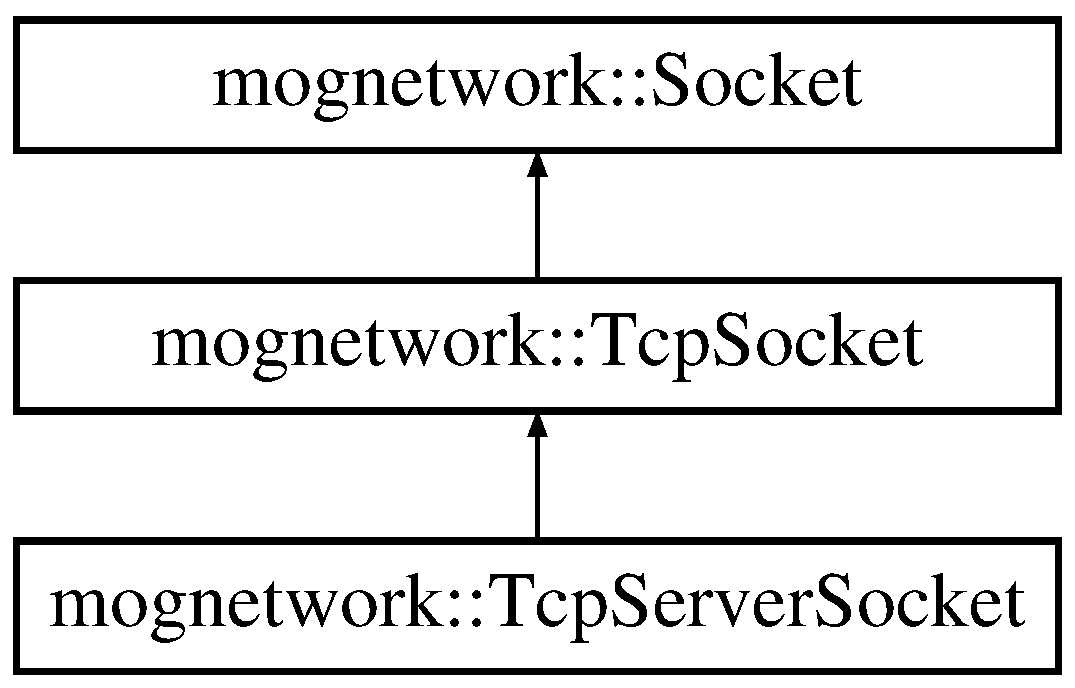
\includegraphics[height=3.000000cm]{classmognetwork_1_1_socket}
\end{center}
\end{figure}
\subsection*{Public Types}
\begin{DoxyCompactItemize}
\item 
enum \hyperlink{classmognetwork_1_1_socket_aa187a8394ac0d6203af0ec7f021ca15f}{Status} \{ \\*
\hyperlink{classmognetwork_1_1_socket_aa187a8394ac0d6203af0ec7f021ca15fa1a76bb652d4c1fdb64829e97b7062a7b}{Ok}, 
\hyperlink{classmognetwork_1_1_socket_aa187a8394ac0d6203af0ec7f021ca15fa088ded708dfc87053ea73283b18929b5}{Nok}, 
\hyperlink{classmognetwork_1_1_socket_aa187a8394ac0d6203af0ec7f021ca15fa76cee46670ca9c26209aaf48ba12a6ea}{Disconnected}, 
\hyperlink{classmognetwork_1_1_socket_aa187a8394ac0d6203af0ec7f021ca15fa73f0c13cec39a68a4896b33c916d551c}{Waiting}, 
\\*
\hyperlink{classmognetwork_1_1_socket_aa187a8394ac0d6203af0ec7f021ca15fae82858abe36f6f41dde52bea32212238}{Error}
 \}
\begin{DoxyCompactList}\small\item\em Définit les status possibles d'une socket. \end{DoxyCompactList}\end{DoxyCompactItemize}
\subsection*{Public Member Functions}
\begin{DoxyCompactItemize}
\item 
Socket\-F\-D \hyperlink{classmognetwork_1_1_socket_a6fc34e842d4efbd526697a12e826806a}{get\-Socket\-F\-D} () const 
\begin{DoxyCompactList}\small\item\em récupère le F\-D de la socket \end{DoxyCompactList}\end{DoxyCompactItemize}
\subsection*{Protected Types}
\begin{DoxyCompactItemize}
\item 
enum \hyperlink{classmognetwork_1_1_socket_a70fb1fd697cfe89987e81bbe9db8ea4d}{Type} \{ \hyperlink{classmognetwork_1_1_socket_a70fb1fd697cfe89987e81bbe9db8ea4dad6adab633c51e7fd9780763f821bea67}{Tcp}, 
\hyperlink{classmognetwork_1_1_socket_a70fb1fd697cfe89987e81bbe9db8ea4dac91debddee39f30455177839f94bdde6}{Udp}
 \}
\begin{DoxyCompactList}\small\item\em Définit le type de socket. \end{DoxyCompactList}\end{DoxyCompactItemize}
\subsection*{Protected Member Functions}
\begin{DoxyCompactItemize}
\item 
\hyperlink{classmognetwork_1_1_socket_a27ed1b1c76de76da577ccbf5b0b687ef}{Socket} (\hyperlink{classmognetwork_1_1_socket_a70fb1fd697cfe89987e81bbe9db8ea4d}{Type} type)
\begin{DoxyCompactList}\small\item\em Constructeur de la socket. \end{DoxyCompactList}\item 
\hypertarget{classmognetwork_1_1_socket_a442e315822bc0fbeeb7c5669a0dceacc}{void \hyperlink{classmognetwork_1_1_socket_a442e315822bc0fbeeb7c5669a0dceacc}{create} ()}\label{classmognetwork_1_1_socket_a442e315822bc0fbeeb7c5669a0dceacc}

\begin{DoxyCompactList}\small\item\em crée la socket et crée un F\-D \end{DoxyCompactList}\item 
\hypertarget{classmognetwork_1_1_socket_a60e3f8b01b89ba0ce03c24ac92e4be0d}{void \hyperlink{classmognetwork_1_1_socket_a60e3f8b01b89ba0ce03c24ac92e4be0d}{create} (Socket\-F\-D fd)}\label{classmognetwork_1_1_socket_a60e3f8b01b89ba0ce03c24ac92e4be0d}

\begin{DoxyCompactList}\small\item\em crée la socket via un F\-D déjà ouvert \end{DoxyCompactList}\item 
\hypertarget{classmognetwork_1_1_socket_a7e8f6bc7f729be6cf1d8c1d5dd638a0b}{void \hyperlink{classmognetwork_1_1_socket_a7e8f6bc7f729be6cf1d8c1d5dd638a0b}{close} ()}\label{classmognetwork_1_1_socket_a7e8f6bc7f729be6cf1d8c1d5dd638a0b}

\begin{DoxyCompactList}\small\item\em ferme la socket \end{DoxyCompactList}\end{DoxyCompactItemize}


\subsection{Detailed Description}
Définit la base d'une socket. 

\subsection{Member Enumeration Documentation}
\hypertarget{classmognetwork_1_1_socket_aa187a8394ac0d6203af0ec7f021ca15f}{\index{mognetwork\-::\-Socket@{mognetwork\-::\-Socket}!Status@{Status}}
\index{Status@{Status}!mognetwork::Socket@{mognetwork\-::\-Socket}}
\subsubsection[{Status}]{\setlength{\rightskip}{0pt plus 5cm}enum {\bf mognetwork\-::\-Socket\-::\-Status}}}\label{classmognetwork_1_1_socket_aa187a8394ac0d6203af0ec7f021ca15f}


Définit les status possibles d'une socket. 

\begin{Desc}
\item[Enumerator]\par
\begin{description}
\index{Ok@{Ok}!mognetwork\-::\-Socket@{mognetwork\-::\-Socket}}\index{mognetwork\-::\-Socket@{mognetwork\-::\-Socket}!Ok@{Ok}}\item[{\em 
\hypertarget{classmognetwork_1_1_socket_aa187a8394ac0d6203af0ec7f021ca15fa1a76bb652d4c1fdb64829e97b7062a7b}{Ok}\label{classmognetwork_1_1_socket_aa187a8394ac0d6203af0ec7f021ca15fa1a76bb652d4c1fdb64829e97b7062a7b}
}]\hyperlink{classmognetwork_1_1_socket}{Socket} prête à la lecture/écriture \index{Nok@{Nok}!mognetwork\-::\-Socket@{mognetwork\-::\-Socket}}\index{mognetwork\-::\-Socket@{mognetwork\-::\-Socket}!Nok@{Nok}}\item[{\em 
\hypertarget{classmognetwork_1_1_socket_aa187a8394ac0d6203af0ec7f021ca15fa088ded708dfc87053ea73283b18929b5}{Nok}\label{classmognetwork_1_1_socket_aa187a8394ac0d6203af0ec7f021ca15fa088ded708dfc87053ea73283b18929b5}
}]\hyperlink{classmognetwork_1_1_socket}{Socket} non prête à la lecture/écriture \index{Disconnected@{Disconnected}!mognetwork\-::\-Socket@{mognetwork\-::\-Socket}}\index{mognetwork\-::\-Socket@{mognetwork\-::\-Socket}!Disconnected@{Disconnected}}\item[{\em 
\hypertarget{classmognetwork_1_1_socket_aa187a8394ac0d6203af0ec7f021ca15fa76cee46670ca9c26209aaf48ba12a6ea}{Disconnected}\label{classmognetwork_1_1_socket_aa187a8394ac0d6203af0ec7f021ca15fa76cee46670ca9c26209aaf48ba12a6ea}
}]\hyperlink{classmognetwork_1_1_socket}{Socket} déconnectée \index{Waiting@{Waiting}!mognetwork\-::\-Socket@{mognetwork\-::\-Socket}}\index{mognetwork\-::\-Socket@{mognetwork\-::\-Socket}!Waiting@{Waiting}}\item[{\em 
\hypertarget{classmognetwork_1_1_socket_aa187a8394ac0d6203af0ec7f021ca15fa73f0c13cec39a68a4896b33c916d551c}{Waiting}\label{classmognetwork_1_1_socket_aa187a8394ac0d6203af0ec7f021ca15fa73f0c13cec39a68a4896b33c916d551c}
}]Attente de données \index{Error@{Error}!mognetwork\-::\-Socket@{mognetwork\-::\-Socket}}\index{mognetwork\-::\-Socket@{mognetwork\-::\-Socket}!Error@{Error}}\item[{\em 
\hypertarget{classmognetwork_1_1_socket_aa187a8394ac0d6203af0ec7f021ca15fae82858abe36f6f41dde52bea32212238}{Error}\label{classmognetwork_1_1_socket_aa187a8394ac0d6203af0ec7f021ca15fae82858abe36f6f41dde52bea32212238}
}]Erreur inconnue \end{description}
\end{Desc}
\hypertarget{classmognetwork_1_1_socket_a70fb1fd697cfe89987e81bbe9db8ea4d}{\index{mognetwork\-::\-Socket@{mognetwork\-::\-Socket}!Type@{Type}}
\index{Type@{Type}!mognetwork::Socket@{mognetwork\-::\-Socket}}
\subsubsection[{Type}]{\setlength{\rightskip}{0pt plus 5cm}enum {\bf mognetwork\-::\-Socket\-::\-Type}\hspace{0.3cm}{\ttfamily [protected]}}}\label{classmognetwork_1_1_socket_a70fb1fd697cfe89987e81bbe9db8ea4d}


Définit le type de socket. 

\begin{Desc}
\item[Enumerator]\par
\begin{description}
\index{Tcp@{Tcp}!mognetwork\-::\-Socket@{mognetwork\-::\-Socket}}\index{mognetwork\-::\-Socket@{mognetwork\-::\-Socket}!Tcp@{Tcp}}\item[{\em 
\hypertarget{classmognetwork_1_1_socket_a70fb1fd697cfe89987e81bbe9db8ea4dad6adab633c51e7fd9780763f821bea67}{Tcp}\label{classmognetwork_1_1_socket_a70fb1fd697cfe89987e81bbe9db8ea4dad6adab633c51e7fd9780763f821bea67}
}]\hyperlink{classmognetwork_1_1_socket}{Socket} T\-C\-P \index{Udp@{Udp}!mognetwork\-::\-Socket@{mognetwork\-::\-Socket}}\index{mognetwork\-::\-Socket@{mognetwork\-::\-Socket}!Udp@{Udp}}\item[{\em 
\hypertarget{classmognetwork_1_1_socket_a70fb1fd697cfe89987e81bbe9db8ea4dac91debddee39f30455177839f94bdde6}{Udp}\label{classmognetwork_1_1_socket_a70fb1fd697cfe89987e81bbe9db8ea4dac91debddee39f30455177839f94bdde6}
}]\hyperlink{classmognetwork_1_1_socket}{Socket} U\-D\-P \end{description}
\end{Desc}


\subsection{Constructor \& Destructor Documentation}
\hypertarget{classmognetwork_1_1_socket_a27ed1b1c76de76da577ccbf5b0b687ef}{\index{mognetwork\-::\-Socket@{mognetwork\-::\-Socket}!Socket@{Socket}}
\index{Socket@{Socket}!mognetwork::Socket@{mognetwork\-::\-Socket}}
\subsubsection[{Socket}]{\setlength{\rightskip}{0pt plus 5cm}mognetwork\-::\-Socket\-::\-Socket (
\begin{DoxyParamCaption}
\item[{{\bf Type}}]{type}
\end{DoxyParamCaption}
)\hspace{0.3cm}{\ttfamily [protected]}}}\label{classmognetwork_1_1_socket_a27ed1b1c76de76da577ccbf5b0b687ef}


Constructeur de la socket. 


\begin{DoxyParams}{Parameters}
{\em type} & Le type de socket \\
\hline
\end{DoxyParams}


\subsection{Member Function Documentation}
\hypertarget{classmognetwork_1_1_socket_a6fc34e842d4efbd526697a12e826806a}{\index{mognetwork\-::\-Socket@{mognetwork\-::\-Socket}!get\-Socket\-F\-D@{get\-Socket\-F\-D}}
\index{get\-Socket\-F\-D@{get\-Socket\-F\-D}!mognetwork::Socket@{mognetwork\-::\-Socket}}
\subsubsection[{get\-Socket\-F\-D}]{\setlength{\rightskip}{0pt plus 5cm}Socket\-F\-D mognetwork\-::\-Socket\-::get\-Socket\-F\-D (
\begin{DoxyParamCaption}
{}
\end{DoxyParamCaption}
) const}}\label{classmognetwork_1_1_socket_a6fc34e842d4efbd526697a12e826806a}


récupère le F\-D de la socket 

\begin{DoxyReturn}{Returns}
le F\-D de la socket 
\end{DoxyReturn}


The documentation for this class was generated from the following file\-:\begin{DoxyCompactItemize}
\item 
include/\hyperlink{_socket_8hh}{Socket.\-hh}\end{DoxyCompactItemize}

\hypertarget{classmognetwork_1_1_socket_selector}{\section{mognetwork\-:\-:Socket\-Selector Class Reference}
\label{classmognetwork_1_1_socket_selector}\index{mognetwork\-::\-Socket\-Selector@{mognetwork\-::\-Socket\-Selector}}
}
\subsection*{Public Types}
\begin{DoxyCompactItemize}
\item 
enum {\bfseries Trigger\-Type} \{ {\bfseries None}, 
{\bfseries Read}, 
{\bfseries Write}
 \}
\item 
enum {\bfseries State} \{ {\bfseries Waiting}, 
{\bfseries Error}
 \}
\end{DoxyCompactItemize}
\subsection*{Public Member Functions}
\begin{DoxyCompactItemize}
\item 
\hypertarget{classmognetwork_1_1_socket_selector_ac8234852e4c0331bda4bb6f7652fc577}{{\bfseries Socket\-Selector} (\hyperlink{classmognetwork_1_1_tcp_socket}{Tcp\-Socket} \&server\-Socket, \hyperlink{classmognetwork_1_1_socket_selector_listener}{Socket\-Selector\-Listener} \&socket\-Selector\-Listener)}\label{classmognetwork_1_1_socket_selector_ac8234852e4c0331bda4bb6f7652fc577}

\item 
\hypertarget{classmognetwork_1_1_socket_selector_a3fe05bc9c20816c29cf37bc7be726c33}{void {\bfseries wait\-For\-Trigger} ()}\label{classmognetwork_1_1_socket_selector_a3fe05bc9c20816c29cf37bc7be726c33}

\item 
\hypertarget{classmognetwork_1_1_socket_selector_a9faab8e39bb69a7812f7cffc1a1df8bf}{void {\bfseries set\-Timeout} (\hyperlink{_selector_8hh_af47ac292ef7224cf549b944d138ba4ae}{Time} $\ast$timeout)}\label{classmognetwork_1_1_socket_selector_a9faab8e39bb69a7812f7cffc1a1df8bf}

\item 
\hypertarget{classmognetwork_1_1_socket_selector_a2f3b8e6214ddd0568182a49080cbd4bf}{\hyperlink{_selector_8hh_af47ac292ef7224cf549b944d138ba4ae}{Time} $\ast$ {\bfseries get\-Timeout} () const }\label{classmognetwork_1_1_socket_selector_a2f3b8e6214ddd0568182a49080cbd4bf}

\item 
\hypertarget{classmognetwork_1_1_socket_selector_a3403ba6262684fdabb84d67788bd5498}{State {\bfseries get\-State} () const }\label{classmognetwork_1_1_socket_selector_a3403ba6262684fdabb84d67788bd5498}

\item 
\hypertarget{classmognetwork_1_1_socket_selector_a0703a1875f67597993b4291119171197}{const \hyperlink{classmognetwork_1_1_tcp_socket}{Tcp\-Socket} \& {\bfseries get\-Server\-Socket} () const }\label{classmognetwork_1_1_socket_selector_a0703a1875f67597993b4291119171197}

\end{DoxyCompactItemize}


The documentation for this class was generated from the following file\-:\begin{DoxyCompactItemize}
\item 
include/\hyperlink{_socket_selector_8hh}{Socket\-Selector.\-hh}\end{DoxyCompactItemize}

\hypertarget{classmognetwork_1_1_socket_selector_listener}{\section{mognetwork\-:\-:Socket\-Selector\-Listener Class Reference}
\label{classmognetwork_1_1_socket_selector_listener}\index{mognetwork\-::\-Socket\-Selector\-Listener@{mognetwork\-::\-Socket\-Selector\-Listener}}
}
\subsection*{Public Member Functions}
\begin{DoxyCompactItemize}
\item 
\hypertarget{classmognetwork_1_1_socket_selector_listener_a5940a832d52941961c2361d950c9bfc1}{virtual void {\bfseries client\-Accepted} (\hyperlink{classmognetwork_1_1_tcp_socket}{Tcp\-Socket} \&client)}\label{classmognetwork_1_1_socket_selector_listener_a5940a832d52941961c2361d950c9bfc1}

\item 
\hypertarget{classmognetwork_1_1_socket_selector_listener_a9219c1c75802958e552fb2b96636200b}{virtual void {\bfseries client\-Datas\-Received} (\hyperlink{classmognetwork_1_1_tcp_socket}{Tcp\-Socket} \&client)}\label{classmognetwork_1_1_socket_selector_listener_a9219c1c75802958e552fb2b96636200b}

\item 
\hypertarget{classmognetwork_1_1_socket_selector_listener_a094cfb5ddd27825e98ebecc10990218d}{virtual void {\bfseries client\-Disconnected} (\hyperlink{classmognetwork_1_1_tcp_socket}{Tcp\-Socket} \&client)}\label{classmognetwork_1_1_socket_selector_listener_a094cfb5ddd27825e98ebecc10990218d}

\end{DoxyCompactItemize}


The documentation for this class was generated from the following file\-:\begin{DoxyCompactItemize}
\item 
include/\hyperlink{_socket_selector_listener_8hh}{Socket\-Selector\-Listener.\-hh}\end{DoxyCompactItemize}

\hypertarget{classmognetwork_1_1_tcp_a_s_i_o_listener}{\section{mognetwork\-:\-:Tcp\-A\-S\-I\-O\-Listener Class Reference}
\label{classmognetwork_1_1_tcp_a_s_i_o_listener}\index{mognetwork\-::\-Tcp\-A\-S\-I\-O\-Listener@{mognetwork\-::\-Tcp\-A\-S\-I\-O\-Listener}}
}


Permet la gestion de la lecture de données en A\-S\-I\-O.  




{\ttfamily \#include $<$Tcp\-A\-S\-I\-O\-Listener.\-hh$>$}

Inheritance diagram for mognetwork\-:\-:Tcp\-A\-S\-I\-O\-Listener\-:\begin{figure}[H]
\begin{center}
\leavevmode
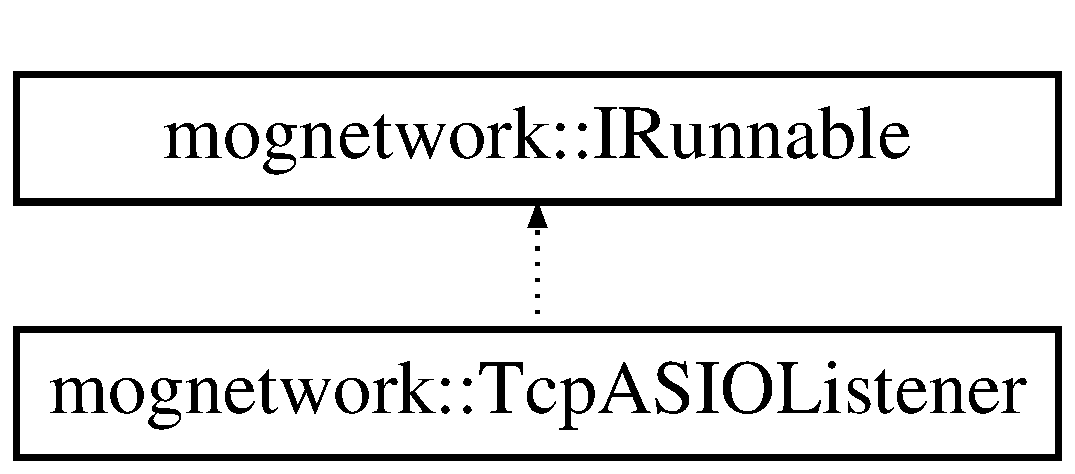
\includegraphics[height=2.000000cm]{classmognetwork_1_1_tcp_a_s_i_o_listener}
\end{center}
\end{figure}
\subsection*{Public Member Functions}
\begin{DoxyCompactItemize}
\item 
\hyperlink{classmognetwork_1_1_tcp_a_s_i_o_listener_aae7628471fda37905fab2dc03db11f77}{Tcp\-A\-S\-I\-O\-Listener} (\hyperlink{classmognetwork_1_1_tcp_server_socket}{Tcp\-Server\-Socket} \&server\-Socket)
\begin{DoxyCompactList}\small\item\em constructeur par défaut \end{DoxyCompactList}\item 
\hypertarget{classmognetwork_1_1_tcp_a_s_i_o_listener_afd805699dfe27ceb0541feeefacc13dc}{void \hyperlink{classmognetwork_1_1_tcp_a_s_i_o_listener_afd805699dfe27ceb0541feeefacc13dc}{start} ()}\label{classmognetwork_1_1_tcp_a_s_i_o_listener_afd805699dfe27ceb0541feeefacc13dc}

\begin{DoxyCompactList}\small\item\em Démarre le thread d'écoute. \end{DoxyCompactList}\item 
\hypertarget{classmognetwork_1_1_tcp_a_s_i_o_listener_ac9952961dce0f44bc720485a4e4e620d}{void \hyperlink{classmognetwork_1_1_tcp_a_s_i_o_listener_ac9952961dce0f44bc720485a4e4e620d}{stop} ()}\label{classmognetwork_1_1_tcp_a_s_i_o_listener_ac9952961dce0f44bc720485a4e4e620d}

\begin{DoxyCompactList}\small\item\em Arrête le thread d'écoute. \end{DoxyCompactList}\item 
\hypertarget{classmognetwork_1_1_tcp_a_s_i_o_listener_ae6327f6471291ba5107c0a9c3362b929}{void \hyperlink{classmognetwork_1_1_tcp_a_s_i_o_listener_ae6327f6471291ba5107c0a9c3362b929}{wait} ()}\label{classmognetwork_1_1_tcp_a_s_i_o_listener_ae6327f6471291ba5107c0a9c3362b929}

\begin{DoxyCompactList}\small\item\em Permet d'attendre la fin de l'exécution du thread d'écoute. \end{DoxyCompactList}\item 
void \hyperlink{classmognetwork_1_1_tcp_a_s_i_o_listener_a0d0b24852fdd94ad5096a87a40bc7712}{add\-Listener} (\hyperlink{classmognetwork_1_1_i_tcp_a_s_i_o_listener_handler}{I\-Tcp\-A\-S\-I\-O\-Listener\-Handler} $\ast$listener)
\begin{DoxyCompactList}\small\item\em Ajoute un listener au thread d'écoute. \end{DoxyCompactList}\item 
bool \hyperlink{classmognetwork_1_1_tcp_a_s_i_o_listener_a431eb0fb3fab8042a9ef0b79d706fffc}{is\-Running} () const 
\begin{DoxyCompactList}\small\item\em Permet de savoir si le thread est démarré \end{DoxyCompactList}\item 
\hypertarget{classmognetwork_1_1_tcp_a_s_i_o_listener_a445dcd4bf6dfe75c7715af0fecf9494d}{void \hyperlink{classmognetwork_1_1_tcp_a_s_i_o_listener_a445dcd4bf6dfe75c7715af0fecf9494d}{run} ()}\label{classmognetwork_1_1_tcp_a_s_i_o_listener_a445dcd4bf6dfe75c7715af0fecf9494d}

\begin{DoxyCompactList}\small\item\em Utilisé par le thread. \hyperlink{classmognetwork_1_1_i_runnable}{I\-Runnable}. \end{DoxyCompactList}\item 
\hyperlink{classmognetwork_1_1_selector}{Selector} \& \hyperlink{classmognetwork_1_1_tcp_a_s_i_o_listener_aed4473511088d8bc91ce118334eed24d}{get\-Selector} ()
\begin{DoxyCompactList}\small\item\em Permet de récupérer une référence sur le selector du thread. \end{DoxyCompactList}\end{DoxyCompactItemize}


\subsection{Detailed Description}
Permet la gestion de la lecture de données en A\-S\-I\-O. 

\subsection{Constructor \& Destructor Documentation}
\hypertarget{classmognetwork_1_1_tcp_a_s_i_o_listener_aae7628471fda37905fab2dc03db11f77}{\index{mognetwork\-::\-Tcp\-A\-S\-I\-O\-Listener@{mognetwork\-::\-Tcp\-A\-S\-I\-O\-Listener}!Tcp\-A\-S\-I\-O\-Listener@{Tcp\-A\-S\-I\-O\-Listener}}
\index{Tcp\-A\-S\-I\-O\-Listener@{Tcp\-A\-S\-I\-O\-Listener}!mognetwork::TcpASIOListener@{mognetwork\-::\-Tcp\-A\-S\-I\-O\-Listener}}
\subsubsection[{Tcp\-A\-S\-I\-O\-Listener}]{\setlength{\rightskip}{0pt plus 5cm}mognetwork\-::\-Tcp\-A\-S\-I\-O\-Listener\-::\-Tcp\-A\-S\-I\-O\-Listener (
\begin{DoxyParamCaption}
\item[{{\bf Tcp\-Server\-Socket} \&}]{server\-Socket}
\end{DoxyParamCaption}
)}}\label{classmognetwork_1_1_tcp_a_s_i_o_listener_aae7628471fda37905fab2dc03db11f77}


constructeur par défaut 


\begin{DoxyParams}{Parameters}
{\em server\-Socket} & la socket serveur \\
\hline
\end{DoxyParams}


\subsection{Member Function Documentation}
\hypertarget{classmognetwork_1_1_tcp_a_s_i_o_listener_a0d0b24852fdd94ad5096a87a40bc7712}{\index{mognetwork\-::\-Tcp\-A\-S\-I\-O\-Listener@{mognetwork\-::\-Tcp\-A\-S\-I\-O\-Listener}!add\-Listener@{add\-Listener}}
\index{add\-Listener@{add\-Listener}!mognetwork::TcpASIOListener@{mognetwork\-::\-Tcp\-A\-S\-I\-O\-Listener}}
\subsubsection[{add\-Listener}]{\setlength{\rightskip}{0pt plus 5cm}void mognetwork\-::\-Tcp\-A\-S\-I\-O\-Listener\-::add\-Listener (
\begin{DoxyParamCaption}
\item[{{\bf I\-Tcp\-A\-S\-I\-O\-Listener\-Handler} $\ast$}]{listener}
\end{DoxyParamCaption}
)\hspace{0.3cm}{\ttfamily [inline]}}}\label{classmognetwork_1_1_tcp_a_s_i_o_listener_a0d0b24852fdd94ad5096a87a40bc7712}


Ajoute un listener au thread d'écoute. 


\begin{DoxyParams}{Parameters}
{\em listener} & le listener à ajouter, instance de I\-T\-Cp\-A\-S\-I\-O\-Listener\-Handler \\
\hline
\end{DoxyParams}
\hypertarget{classmognetwork_1_1_tcp_a_s_i_o_listener_aed4473511088d8bc91ce118334eed24d}{\index{mognetwork\-::\-Tcp\-A\-S\-I\-O\-Listener@{mognetwork\-::\-Tcp\-A\-S\-I\-O\-Listener}!get\-Selector@{get\-Selector}}
\index{get\-Selector@{get\-Selector}!mognetwork::TcpASIOListener@{mognetwork\-::\-Tcp\-A\-S\-I\-O\-Listener}}
\subsubsection[{get\-Selector}]{\setlength{\rightskip}{0pt plus 5cm}{\bf Selector}\& mognetwork\-::\-Tcp\-A\-S\-I\-O\-Listener\-::get\-Selector (
\begin{DoxyParamCaption}
{}
\end{DoxyParamCaption}
)\hspace{0.3cm}{\ttfamily [inline]}}}\label{classmognetwork_1_1_tcp_a_s_i_o_listener_aed4473511088d8bc91ce118334eed24d}


Permet de récupérer une référence sur le selector du thread. 

\begin{DoxyReturn}{Returns}
la référence sur le \hyperlink{classmognetwork_1_1_selector}{Selector} 
\end{DoxyReturn}
\hypertarget{classmognetwork_1_1_tcp_a_s_i_o_listener_a431eb0fb3fab8042a9ef0b79d706fffc}{\index{mognetwork\-::\-Tcp\-A\-S\-I\-O\-Listener@{mognetwork\-::\-Tcp\-A\-S\-I\-O\-Listener}!is\-Running@{is\-Running}}
\index{is\-Running@{is\-Running}!mognetwork::TcpASIOListener@{mognetwork\-::\-Tcp\-A\-S\-I\-O\-Listener}}
\subsubsection[{is\-Running}]{\setlength{\rightskip}{0pt plus 5cm}bool mognetwork\-::\-Tcp\-A\-S\-I\-O\-Listener\-::is\-Running (
\begin{DoxyParamCaption}
{}
\end{DoxyParamCaption}
) const\hspace{0.3cm}{\ttfamily [inline]}}}\label{classmognetwork_1_1_tcp_a_s_i_o_listener_a431eb0fb3fab8042a9ef0b79d706fffc}


Permet de savoir si le thread est démarré 

\begin{DoxyReturn}{Returns}
true si démarré, false sinon 
\end{DoxyReturn}


The documentation for this class was generated from the following file\-:\begin{DoxyCompactItemize}
\item 
include/mognetwork/\hyperlink{_tcp_a_s_i_o_listener_8hh}{Tcp\-A\-S\-I\-O\-Listener.\-hh}\end{DoxyCompactItemize}

\hypertarget{classmognetwork_1_1_tcp_socket}{\section{mognetwork\-:\-:Tcp\-Socket Class Reference}
\label{classmognetwork_1_1_tcp_socket}\index{mognetwork\-::\-Tcp\-Socket@{mognetwork\-::\-Tcp\-Socket}}
}


Classe de création d'une socket T\-C\-P.  




{\ttfamily \#include $<$Tcp\-Socket.\-hh$>$}

Inheritance diagram for mognetwork\-:\-:Tcp\-Socket\-:\begin{figure}[H]
\begin{center}
\leavevmode
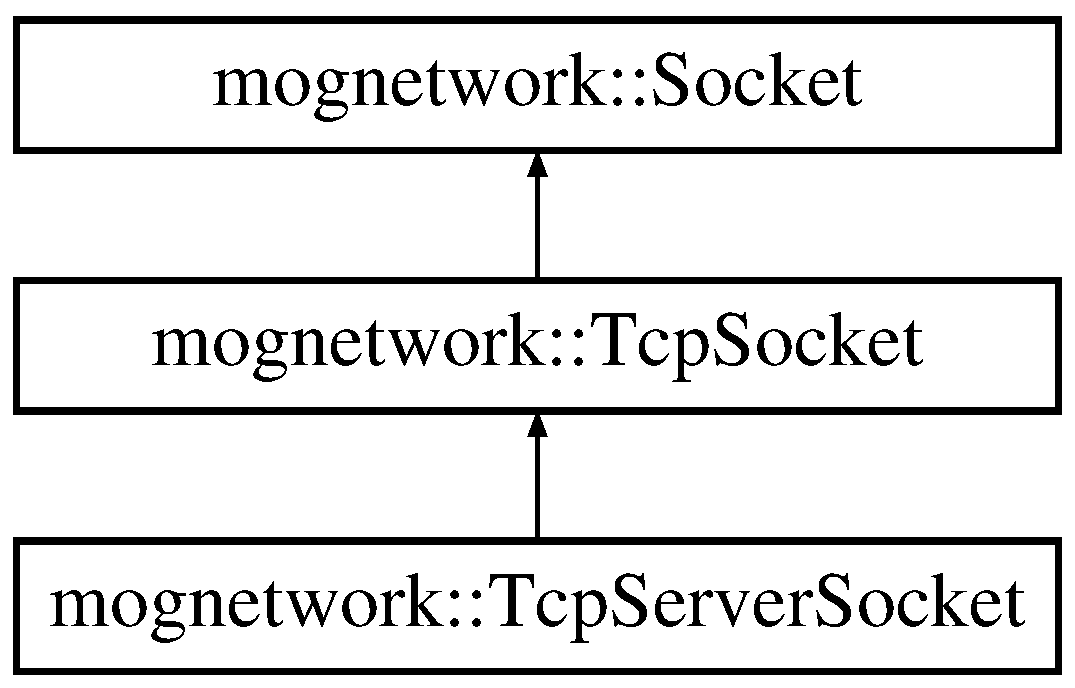
\includegraphics[height=3.000000cm]{classmognetwork_1_1_tcp_socket}
\end{center}
\end{figure}
\subsection*{Classes}
\begin{DoxyCompactItemize}
\item 
struct \hyperlink{structmognetwork_1_1_tcp_socket_1_1_readed_datas}{Readed\-Datas}
\begin{DoxyCompactList}\small\item\em Contient toutes les données relatives à la lecture d'une donnée en réseau. \end{DoxyCompactList}\end{DoxyCompactItemize}
\subsection*{Public Types}
\begin{DoxyCompactItemize}
\item 
typedef std\-::vector$<$ char $>$ \hyperlink{classmognetwork_1_1_tcp_socket_aa80d910649a16cedb6c98297e5893ed1}{Data}
\item 
typedef std\-::list$<$ \hyperlink{classmognetwork_1_1_tcp_socket_aa80d910649a16cedb6c98297e5893ed1}{Data} $>$ \hyperlink{classmognetwork_1_1_tcp_socket_ad7bb1f8749cfba5e4b181b035b0659c1}{Data\-List}
\end{DoxyCompactItemize}
\subsection*{Public Member Functions}
\begin{DoxyCompactItemize}
\item 
\hypertarget{classmognetwork_1_1_tcp_socket_ae3ffb22c96fde72fbf2723c6f250f3be}{\hyperlink{classmognetwork_1_1_tcp_socket_ae3ffb22c96fde72fbf2723c6f250f3be}{Tcp\-Socket} ()}\label{classmognetwork_1_1_tcp_socket_ae3ffb22c96fde72fbf2723c6f250f3be}

\begin{DoxyCompactList}\small\item\em Constructeur d'une socket en T\-C\-P par défaut. \end{DoxyCompactList}\item 
\hyperlink{classmognetwork_1_1_tcp_socket_abd9e4da7abe977703de3d10aa02ec3c0}{Tcp\-Socket} (Socket\-F\-D fd)
\begin{DoxyCompactList}\small\item\em Constructeur d'une socket T\-C\-P à partir d'une socket déjà ouverte. \end{DoxyCompactList}\item 
\hyperlink{classmognetwork_1_1_socket_aa187a8394ac0d6203af0ec7f021ca15f}{Socket\-::\-Status} \hyperlink{classmognetwork_1_1_tcp_socket_a370b1ee9cfd40eb1c8a2a4ee47303363}{connect} (const \hyperlink{classmognetwork_1_1_ip_address}{Ip\-Address} \&address, unsigned short port)
\begin{DoxyCompactList}\small\item\em Connecte la socket à une adresse. \end{DoxyCompactList}\item 
\hypertarget{classmognetwork_1_1_tcp_socket_a4da14b8d1e0f71bfae8c0fe6eb54be19}{void \hyperlink{classmognetwork_1_1_tcp_socket_a4da14b8d1e0f71bfae8c0fe6eb54be19}{disconnect} ()}\label{classmognetwork_1_1_tcp_socket_a4da14b8d1e0f71bfae8c0fe6eb54be19}

\begin{DoxyCompactList}\small\item\em Déconnecte la socket. \end{DoxyCompactList}\item 
\hyperlink{classmognetwork_1_1_socket_aa187a8394ac0d6203af0ec7f021ca15f}{Socket\-::\-Status} \hyperlink{classmognetwork_1_1_tcp_socket_a6cd80d53f05a4d91ed1a66e17e9a3d54}{send} (const char $\ast$data, std\-::size\-\_\-t size)
\begin{DoxyCompactList}\small\item\em Envois des données de manière synchrone (blockante) \end{DoxyCompactList}\item 
\hyperlink{classmognetwork_1_1_socket_aa187a8394ac0d6203af0ec7f021ca15f}{Socket\-::\-Status} \hyperlink{classmognetwork_1_1_tcp_socket_a44fd93d5f7bcf3d155a93e4db6d5f2e9}{receive} (char $\ast$data, std\-::size\-\_\-t size, std\-::size\-\_\-t \&received, int \-\_\-flags)
\begin{DoxyCompactList}\small\item\em Reçoit des données de manière synchrone (blockante) \end{DoxyCompactList}\item 
\hyperlink{classmognetwork_1_1_socket_aa187a8394ac0d6203af0ec7f021ca15f}{Socket\-::\-Status} \hyperlink{classmognetwork_1_1_tcp_socket_ae136e74283e5e8d0704c52d8110f1896}{async\-Send} (const char $\ast$data, std\-::size\-\_\-t size)
\begin{DoxyCompactList}\small\item\em Ajoute des données à la liste d'envois des données de la socket en Asynchrone. \end{DoxyCompactList}\item 
\hyperlink{classmognetwork_1_1_socket_aa187a8394ac0d6203af0ec7f021ca15f}{Socket\-::\-Status} \hyperlink{classmognetwork_1_1_tcp_socket_afbb854293f7f8e404bb553e5c5ba1277}{send\-Pending\-Datas} ()
\begin{DoxyCompactList}\small\item\em Envois les données en attente ajoutées par async\-Send. \end{DoxyCompactList}\item 
bool \hyperlink{classmognetwork_1_1_tcp_socket_aff17b683f622b017876751d9cbbad3bb}{having\-Pending\-Datas} () const 
\begin{DoxyCompactList}\small\item\em Permet de savoir si il reste des données à envoyer via send\-Pending\-Datas. \end{DoxyCompactList}\item 
void \hyperlink{classmognetwork_1_1_tcp_socket_a2d7327be349e705c74bdc6b40c1b2520}{set\-User\-Data} (void $\ast$user\-Data)
\begin{DoxyCompactList}\small\item\em Définit des données pouvant être récupérées via la socket. \end{DoxyCompactList}\item 
void $\ast$ \hyperlink{classmognetwork_1_1_tcp_socket_adef63a929423324fd75888e2195176e0}{get\-User\-Data} () const 
\begin{DoxyCompactList}\small\item\em Récupère des données enregistrées sur la socket. \end{DoxyCompactList}\item 
\hyperlink{classmognetwork_1_1_socket_aa187a8394ac0d6203af0ec7f021ca15f}{Socket\-::\-Status} \hyperlink{classmognetwork_1_1_tcp_socket_af3918374ee41223b77f669367d4b0e22}{read\-Pending\-Datas} ()
\begin{DoxyCompactList}\small\item\em Lis les données en attente en Asynchrone. \end{DoxyCompactList}\item 
const \hyperlink{structmognetwork_1_1_tcp_socket_1_1_readed_datas}{Tcp\-Socket\-::\-Readed\-Datas} $\ast$ \hyperlink{classmognetwork_1_1_tcp_socket_ab9e99c5f8bc2099de32670ff1b7bcaf3}{get\-Datas\-Readed} () const 
\begin{DoxyCompactList}\small\item\em Récupère les données lues via read\-Pending\-Datas. \end{DoxyCompactList}\item 
const \hyperlink{classmognetwork_1_1_packet}{Packet} $\ast$ \hyperlink{classmognetwork_1_1_tcp_socket_a9256f406b68101bee2735f7ecfe104e8}{get\-Packet\-Readed} ()
\begin{DoxyCompactList}\small\item\em Récupère les données lues via read\-Pending\-Datas en temps que \hyperlink{classmognetwork_1_1_packet}{Packet}. \end{DoxyCompactList}\end{DoxyCompactItemize}
\subsection*{Additional Inherited Members}


\subsection{Detailed Description}
Classe de création d'une socket T\-C\-P. 

\subsection{Member Typedef Documentation}
\hypertarget{classmognetwork_1_1_tcp_socket_aa80d910649a16cedb6c98297e5893ed1}{\index{mognetwork\-::\-Tcp\-Socket@{mognetwork\-::\-Tcp\-Socket}!Data@{Data}}
\index{Data@{Data}!mognetwork::TcpSocket@{mognetwork\-::\-Tcp\-Socket}}
\subsubsection[{Data}]{\setlength{\rightskip}{0pt plus 5cm}typedef std\-::vector$<$char$>$ {\bf mognetwork\-::\-Tcp\-Socket\-::\-Data}}}\label{classmognetwork_1_1_tcp_socket_aa80d910649a16cedb6c98297e5893ed1}
Typedef pour définit le typpage d'une Data \hypertarget{classmognetwork_1_1_tcp_socket_ad7bb1f8749cfba5e4b181b035b0659c1}{\index{mognetwork\-::\-Tcp\-Socket@{mognetwork\-::\-Tcp\-Socket}!Data\-List@{Data\-List}}
\index{Data\-List@{Data\-List}!mognetwork::TcpSocket@{mognetwork\-::\-Tcp\-Socket}}
\subsubsection[{Data\-List}]{\setlength{\rightskip}{0pt plus 5cm}typedef std\-::list$<${\bf Data}$>$ {\bf mognetwork\-::\-Tcp\-Socket\-::\-Data\-List}}}\label{classmognetwork_1_1_tcp_socket_ad7bb1f8749cfba5e4b181b035b0659c1}
Typedef pour définit une data\-List 

\subsection{Constructor \& Destructor Documentation}
\hypertarget{classmognetwork_1_1_tcp_socket_abd9e4da7abe977703de3d10aa02ec3c0}{\index{mognetwork\-::\-Tcp\-Socket@{mognetwork\-::\-Tcp\-Socket}!Tcp\-Socket@{Tcp\-Socket}}
\index{Tcp\-Socket@{Tcp\-Socket}!mognetwork::TcpSocket@{mognetwork\-::\-Tcp\-Socket}}
\subsubsection[{Tcp\-Socket}]{\setlength{\rightskip}{0pt plus 5cm}mognetwork\-::\-Tcp\-Socket\-::\-Tcp\-Socket (
\begin{DoxyParamCaption}
\item[{Socket\-F\-D}]{fd}
\end{DoxyParamCaption}
)}}\label{classmognetwork_1_1_tcp_socket_abd9e4da7abe977703de3d10aa02ec3c0}


Constructeur d'une socket T\-C\-P à partir d'une socket déjà ouverte. 


\begin{DoxyParams}{Parameters}
{\em fd} & le F\-D de la socket déjà ouverte \\
\hline
\end{DoxyParams}


\subsection{Member Function Documentation}
\hypertarget{classmognetwork_1_1_tcp_socket_ae136e74283e5e8d0704c52d8110f1896}{\index{mognetwork\-::\-Tcp\-Socket@{mognetwork\-::\-Tcp\-Socket}!async\-Send@{async\-Send}}
\index{async\-Send@{async\-Send}!mognetwork::TcpSocket@{mognetwork\-::\-Tcp\-Socket}}
\subsubsection[{async\-Send}]{\setlength{\rightskip}{0pt plus 5cm}{\bf Socket\-::\-Status} mognetwork\-::\-Tcp\-Socket\-::async\-Send (
\begin{DoxyParamCaption}
\item[{const char $\ast$}]{data, }
\item[{std\-::size\-\_\-t}]{size}
\end{DoxyParamCaption}
)}}\label{classmognetwork_1_1_tcp_socket_ae136e74283e5e8d0704c52d8110f1896}


Ajoute des données à la liste d'envois des données de la socket en Asynchrone. 


\begin{DoxyParams}{Parameters}
{\em data} & Les données à envoyer \\
\hline
{\em size} & la taille totale des données \\
\hline
\end{DoxyParams}
\begin{DoxyReturn}{Returns}
\hyperlink{classmognetwork_1_1_socket_aa187a8394ac0d6203af0ec7f021ca15f}{Socket\-::\-Status} permettant de savoir l'état de l'envois 
\end{DoxyReturn}
\hypertarget{classmognetwork_1_1_tcp_socket_a370b1ee9cfd40eb1c8a2a4ee47303363}{\index{mognetwork\-::\-Tcp\-Socket@{mognetwork\-::\-Tcp\-Socket}!connect@{connect}}
\index{connect@{connect}!mognetwork::TcpSocket@{mognetwork\-::\-Tcp\-Socket}}
\subsubsection[{connect}]{\setlength{\rightskip}{0pt plus 5cm}{\bf Socket\-::\-Status} mognetwork\-::\-Tcp\-Socket\-::connect (
\begin{DoxyParamCaption}
\item[{const {\bf Ip\-Address} \&}]{address, }
\item[{unsigned short}]{port}
\end{DoxyParamCaption}
)}}\label{classmognetwork_1_1_tcp_socket_a370b1ee9cfd40eb1c8a2a4ee47303363}


Connecte la socket à une adresse. 


\begin{DoxyParams}{Parameters}
{\em address} & l'adresse où la socket doit se connecter \\
\hline
{\em port} & le port où la socket doit se connecter \\
\hline
\end{DoxyParams}
\hypertarget{classmognetwork_1_1_tcp_socket_ab9e99c5f8bc2099de32670ff1b7bcaf3}{\index{mognetwork\-::\-Tcp\-Socket@{mognetwork\-::\-Tcp\-Socket}!get\-Datas\-Readed@{get\-Datas\-Readed}}
\index{get\-Datas\-Readed@{get\-Datas\-Readed}!mognetwork::TcpSocket@{mognetwork\-::\-Tcp\-Socket}}
\subsubsection[{get\-Datas\-Readed}]{\setlength{\rightskip}{0pt plus 5cm}const {\bf Tcp\-Socket\-::\-Readed\-Datas}$\ast$ mognetwork\-::\-Tcp\-Socket\-::get\-Datas\-Readed (
\begin{DoxyParamCaption}
{}
\end{DoxyParamCaption}
) const}}\label{classmognetwork_1_1_tcp_socket_ab9e99c5f8bc2099de32670ff1b7bcaf3}


Récupère les données lues via read\-Pending\-Datas. 

\begin{DoxyReturn}{Returns}
Les données lues en temps que \hyperlink{structmognetwork_1_1_tcp_socket_1_1_readed_datas}{Tcp\-Socket\-::\-Readed\-Datas} 
\end{DoxyReturn}
\hypertarget{classmognetwork_1_1_tcp_socket_a9256f406b68101bee2735f7ecfe104e8}{\index{mognetwork\-::\-Tcp\-Socket@{mognetwork\-::\-Tcp\-Socket}!get\-Packet\-Readed@{get\-Packet\-Readed}}
\index{get\-Packet\-Readed@{get\-Packet\-Readed}!mognetwork::TcpSocket@{mognetwork\-::\-Tcp\-Socket}}
\subsubsection[{get\-Packet\-Readed}]{\setlength{\rightskip}{0pt plus 5cm}const {\bf Packet}$\ast$ mognetwork\-::\-Tcp\-Socket\-::get\-Packet\-Readed (
\begin{DoxyParamCaption}
{}
\end{DoxyParamCaption}
)}}\label{classmognetwork_1_1_tcp_socket_a9256f406b68101bee2735f7ecfe104e8}


Récupère les données lues via read\-Pending\-Datas en temps que \hyperlink{classmognetwork_1_1_packet}{Packet}. 

\begin{DoxyReturn}{Returns}
Les données en format \hyperlink{classmognetwork_1_1_packet}{Packet} 
\end{DoxyReturn}
\hypertarget{classmognetwork_1_1_tcp_socket_adef63a929423324fd75888e2195176e0}{\index{mognetwork\-::\-Tcp\-Socket@{mognetwork\-::\-Tcp\-Socket}!get\-User\-Data@{get\-User\-Data}}
\index{get\-User\-Data@{get\-User\-Data}!mognetwork::TcpSocket@{mognetwork\-::\-Tcp\-Socket}}
\subsubsection[{get\-User\-Data}]{\setlength{\rightskip}{0pt plus 5cm}void$\ast$ mognetwork\-::\-Tcp\-Socket\-::get\-User\-Data (
\begin{DoxyParamCaption}
{}
\end{DoxyParamCaption}
) const}}\label{classmognetwork_1_1_tcp_socket_adef63a929423324fd75888e2195176e0}


Récupère des données enregistrées sur la socket. 

\begin{DoxyReturn}{Returns}
pointeur contenant les données 
\end{DoxyReturn}
\hypertarget{classmognetwork_1_1_tcp_socket_aff17b683f622b017876751d9cbbad3bb}{\index{mognetwork\-::\-Tcp\-Socket@{mognetwork\-::\-Tcp\-Socket}!having\-Pending\-Datas@{having\-Pending\-Datas}}
\index{having\-Pending\-Datas@{having\-Pending\-Datas}!mognetwork::TcpSocket@{mognetwork\-::\-Tcp\-Socket}}
\subsubsection[{having\-Pending\-Datas}]{\setlength{\rightskip}{0pt plus 5cm}bool mognetwork\-::\-Tcp\-Socket\-::having\-Pending\-Datas (
\begin{DoxyParamCaption}
{}
\end{DoxyParamCaption}
) const}}\label{classmognetwork_1_1_tcp_socket_aff17b683f622b017876751d9cbbad3bb}


Permet de savoir si il reste des données à envoyer via send\-Pending\-Datas. 

\begin{DoxyReturn}{Returns}
true si il en reste, false sinon 
\end{DoxyReturn}
\hypertarget{classmognetwork_1_1_tcp_socket_af3918374ee41223b77f669367d4b0e22}{\index{mognetwork\-::\-Tcp\-Socket@{mognetwork\-::\-Tcp\-Socket}!read\-Pending\-Datas@{read\-Pending\-Datas}}
\index{read\-Pending\-Datas@{read\-Pending\-Datas}!mognetwork::TcpSocket@{mognetwork\-::\-Tcp\-Socket}}
\subsubsection[{read\-Pending\-Datas}]{\setlength{\rightskip}{0pt plus 5cm}{\bf Socket\-::\-Status} mognetwork\-::\-Tcp\-Socket\-::read\-Pending\-Datas (
\begin{DoxyParamCaption}
{}
\end{DoxyParamCaption}
)}}\label{classmognetwork_1_1_tcp_socket_af3918374ee41223b77f669367d4b0e22}


Lis les données en attente en Asynchrone. 

\begin{DoxyReturn}{Returns}
\hyperlink{classmognetwork_1_1_socket_aa187a8394ac0d6203af0ec7f021ca15f}{Socket\-::\-Status} permettant de savoir l'état de la lecture 
\end{DoxyReturn}
\hypertarget{classmognetwork_1_1_tcp_socket_a44fd93d5f7bcf3d155a93e4db6d5f2e9}{\index{mognetwork\-::\-Tcp\-Socket@{mognetwork\-::\-Tcp\-Socket}!receive@{receive}}
\index{receive@{receive}!mognetwork::TcpSocket@{mognetwork\-::\-Tcp\-Socket}}
\subsubsection[{receive}]{\setlength{\rightskip}{0pt plus 5cm}{\bf Socket\-::\-Status} mognetwork\-::\-Tcp\-Socket\-::receive (
\begin{DoxyParamCaption}
\item[{char $\ast$}]{data, }
\item[{std\-::size\-\_\-t}]{size, }
\item[{std\-::size\-\_\-t \&}]{received, }
\item[{int}]{\-\_\-flags}
\end{DoxyParamCaption}
)}}\label{classmognetwork_1_1_tcp_socket_a44fd93d5f7bcf3d155a93e4db6d5f2e9}


Reçoit des données de manière synchrone (blockante) 

\begin{DoxyReturn}{Returns}
\hyperlink{classmognetwork_1_1_socket_aa187a8394ac0d6203af0ec7f021ca15f}{Socket\-::\-Status} permettant de savoir l'état de la réception 
\end{DoxyReturn}
\hypertarget{classmognetwork_1_1_tcp_socket_a6cd80d53f05a4d91ed1a66e17e9a3d54}{\index{mognetwork\-::\-Tcp\-Socket@{mognetwork\-::\-Tcp\-Socket}!send@{send}}
\index{send@{send}!mognetwork::TcpSocket@{mognetwork\-::\-Tcp\-Socket}}
\subsubsection[{send}]{\setlength{\rightskip}{0pt plus 5cm}{\bf Socket\-::\-Status} mognetwork\-::\-Tcp\-Socket\-::send (
\begin{DoxyParamCaption}
\item[{const char $\ast$}]{data, }
\item[{std\-::size\-\_\-t}]{size}
\end{DoxyParamCaption}
)}}\label{classmognetwork_1_1_tcp_socket_a6cd80d53f05a4d91ed1a66e17e9a3d54}


Envois des données de manière synchrone (blockante) 

\begin{DoxyReturn}{Returns}
\hyperlink{classmognetwork_1_1_socket_aa187a8394ac0d6203af0ec7f021ca15f}{Socket\-::\-Status} permettant de savoir l'état de l'envois 
\end{DoxyReturn}
\hypertarget{classmognetwork_1_1_tcp_socket_afbb854293f7f8e404bb553e5c5ba1277}{\index{mognetwork\-::\-Tcp\-Socket@{mognetwork\-::\-Tcp\-Socket}!send\-Pending\-Datas@{send\-Pending\-Datas}}
\index{send\-Pending\-Datas@{send\-Pending\-Datas}!mognetwork::TcpSocket@{mognetwork\-::\-Tcp\-Socket}}
\subsubsection[{send\-Pending\-Datas}]{\setlength{\rightskip}{0pt plus 5cm}{\bf Socket\-::\-Status} mognetwork\-::\-Tcp\-Socket\-::send\-Pending\-Datas (
\begin{DoxyParamCaption}
{}
\end{DoxyParamCaption}
)}}\label{classmognetwork_1_1_tcp_socket_afbb854293f7f8e404bb553e5c5ba1277}


Envois les données en attente ajoutées par async\-Send. 

\begin{DoxyReturn}{Returns}
\hyperlink{classmognetwork_1_1_socket_aa187a8394ac0d6203af0ec7f021ca15f}{Socket\-::\-Status} permettant de savoir l'état de l'envois 
\end{DoxyReturn}
\hypertarget{classmognetwork_1_1_tcp_socket_a2d7327be349e705c74bdc6b40c1b2520}{\index{mognetwork\-::\-Tcp\-Socket@{mognetwork\-::\-Tcp\-Socket}!set\-User\-Data@{set\-User\-Data}}
\index{set\-User\-Data@{set\-User\-Data}!mognetwork::TcpSocket@{mognetwork\-::\-Tcp\-Socket}}
\subsubsection[{set\-User\-Data}]{\setlength{\rightskip}{0pt plus 5cm}void mognetwork\-::\-Tcp\-Socket\-::set\-User\-Data (
\begin{DoxyParamCaption}
\item[{void $\ast$}]{user\-Data}
\end{DoxyParamCaption}
)}}\label{classmognetwork_1_1_tcp_socket_a2d7327be349e705c74bdc6b40c1b2520}


Définit des données pouvant être récupérées via la socket. 


\begin{DoxyParams}{Parameters}
{\em user\-Data} & les données en question \\
\hline
\end{DoxyParams}


The documentation for this class was generated from the following file\-:\begin{DoxyCompactItemize}
\item 
include/\hyperlink{_tcp_socket_8hh}{Tcp\-Socket.\-hh}\end{DoxyCompactItemize}

\hypertarget{classmognetwork_1_1_thread}{\section{mognetwork\-:\-:Thread Class Reference}
\label{classmognetwork_1_1_thread}\index{mognetwork\-::\-Thread@{mognetwork\-::\-Thread}}
}


Classe d'encapsulation des threads.  




{\ttfamily \#include $<$Thread.\-hh$>$}

\subsection*{Public Member Functions}
\begin{DoxyCompactItemize}
\item 
\hyperlink{classmognetwork_1_1_thread_af62df267bb08a768111b98e46b9d8675}{Thread} (\hyperlink{classmognetwork_1_1_i_runnable}{I\-Runnable} \&runnable, bool detach)
\begin{DoxyCompactList}\small\item\em Constructeur. \end{DoxyCompactList}\item 
\hypertarget{classmognetwork_1_1_thread_af50e944ca134178706495a3448a263fc}{virtual void \hyperlink{classmognetwork_1_1_thread_af50e944ca134178706495a3448a263fc}{start} ()}\label{classmognetwork_1_1_thread_af50e944ca134178706495a3448a263fc}

\begin{DoxyCompactList}\small\item\em Lance le thread. \end{DoxyCompactList}\item 
\hypertarget{classmognetwork_1_1_thread_a62e7929cde1edc54df6e4a32bc6dac15}{virtual void \hyperlink{classmognetwork_1_1_thread_a62e7929cde1edc54df6e4a32bc6dac15}{cancel} ()}\label{classmognetwork_1_1_thread_a62e7929cde1edc54df6e4a32bc6dac15}

\begin{DoxyCompactList}\small\item\em Annule le thread. \end{DoxyCompactList}\item 
\hypertarget{classmognetwork_1_1_thread_adc557095ab8d062aad0cbd91e5c5e6ea}{virtual void \hyperlink{classmognetwork_1_1_thread_adc557095ab8d062aad0cbd91e5c5e6ea}{join} ()}\label{classmognetwork_1_1_thread_adc557095ab8d062aad0cbd91e5c5e6ea}

\begin{DoxyCompactList}\small\item\em Attend que le thread se termine. \end{DoxyCompactList}\item 
bool \hyperlink{classmognetwork_1_1_thread_ac980f839f427ef11c0ae74ba5bec9c24}{is\-Started} () const 
\begin{DoxyCompactList}\small\item\em permet de savoir si le thread est actuellement lancé \end{DoxyCompactList}\end{DoxyCompactItemize}
\subsection*{Static Protected Member Functions}
\begin{DoxyCompactItemize}
\item 
\hypertarget{classmognetwork_1_1_thread_add55678bd19ffc48896e36b7ab642113}{static void $\ast$ \hyperlink{classmognetwork_1_1_thread_add55678bd19ffc48896e36b7ab642113}{exec} (void $\ast$)}\label{classmognetwork_1_1_thread_add55678bd19ffc48896e36b7ab642113}

\begin{DoxyCompactList}\small\item\em Utilisée pour passer un pointeur sur fonction au thread. \end{DoxyCompactList}\end{DoxyCompactItemize}


\subsection{Detailed Description}
Classe d'encapsulation des threads. 

\subsection{Constructor \& Destructor Documentation}
\hypertarget{classmognetwork_1_1_thread_af62df267bb08a768111b98e46b9d8675}{\index{mognetwork\-::\-Thread@{mognetwork\-::\-Thread}!Thread@{Thread}}
\index{Thread@{Thread}!mognetwork::Thread@{mognetwork\-::\-Thread}}
\subsubsection[{Thread}]{\setlength{\rightskip}{0pt plus 5cm}mognetwork\-::\-Thread\-::\-Thread (
\begin{DoxyParamCaption}
\item[{{\bf I\-Runnable} \&}]{runnable, }
\item[{bool}]{detach}
\end{DoxyParamCaption}
)}}\label{classmognetwork_1_1_thread_af62df267bb08a768111b98e46b9d8675}


Constructeur. 


\begin{DoxyParams}{Parameters}
{\em runnable} & Un runnable pour le lancement du thread \\
\hline
{\em detach} & Le thread est il attaché? \\
\hline
\end{DoxyParams}


\subsection{Member Function Documentation}
\hypertarget{classmognetwork_1_1_thread_ac980f839f427ef11c0ae74ba5bec9c24}{\index{mognetwork\-::\-Thread@{mognetwork\-::\-Thread}!is\-Started@{is\-Started}}
\index{is\-Started@{is\-Started}!mognetwork::Thread@{mognetwork\-::\-Thread}}
\subsubsection[{is\-Started}]{\setlength{\rightskip}{0pt plus 5cm}bool mognetwork\-::\-Thread\-::is\-Started (
\begin{DoxyParamCaption}
{}
\end{DoxyParamCaption}
) const\hspace{0.3cm}{\ttfamily [inline]}}}\label{classmognetwork_1_1_thread_ac980f839f427ef11c0ae74ba5bec9c24}


permet de savoir si le thread est actuellement lancé 

\begin{DoxyReturn}{Returns}
true si lancé, sinon false 
\end{DoxyReturn}


The documentation for this class was generated from the following file\-:\begin{DoxyCompactItemize}
\item 
include/\hyperlink{_thread_8hh}{Thread.\-hh}\end{DoxyCompactItemize}

\hypertarget{classmognetwork_1_1_thread_exception}{\section{mognetwork\-:\-:Thread\-Exception Class Reference}
\label{classmognetwork_1_1_thread_exception}\index{mognetwork\-::\-Thread\-Exception@{mognetwork\-::\-Thread\-Exception}}
}


\hyperlink{classmognetwork_1_1_thread}{Thread} exceptions class.  




{\ttfamily \#include $<$Thread\-Exception.\-hh$>$}

Inheritance diagram for mognetwork\-:\-:Thread\-Exception\-:\begin{figure}[H]
\begin{center}
\leavevmode
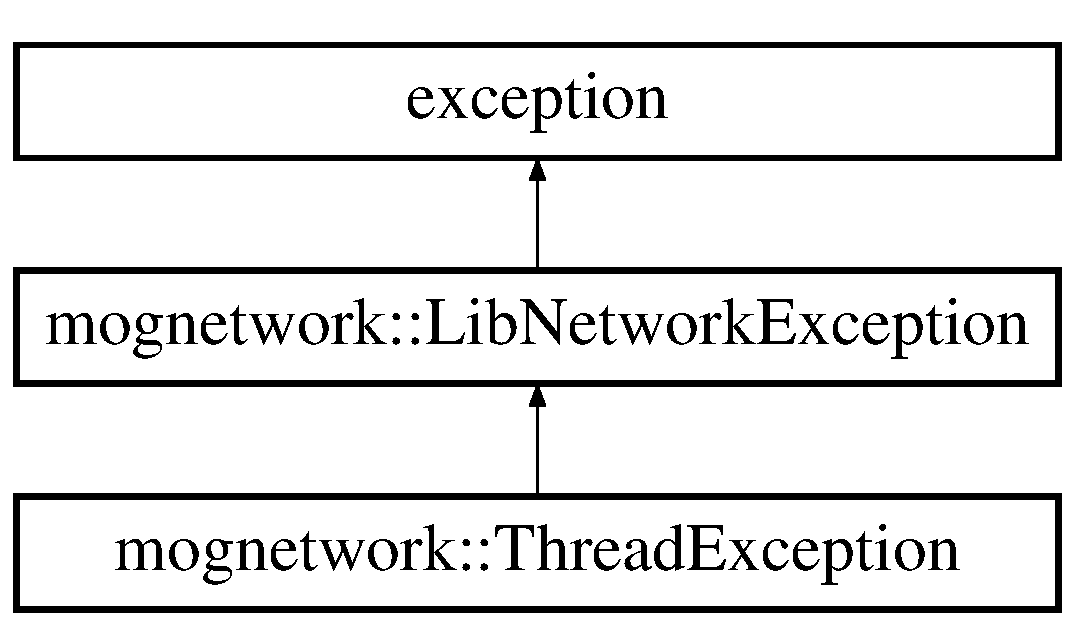
\includegraphics[height=3.000000cm]{classmognetwork_1_1_thread_exception}
\end{center}
\end{figure}
\subsection*{Public Member Functions}
\begin{DoxyCompactItemize}
\item 
\hyperlink{classmognetwork_1_1_thread_exception_a0f8e6b5811c083a0a656e9075fb53674}{Thread\-Exception} (const char $\ast$msg, int line, const char $\ast$file)
\begin{DoxyCompactList}\small\item\em Default constructor. \end{DoxyCompactList}\end{DoxyCompactItemize}


\subsection{Detailed Description}
\hyperlink{classmognetwork_1_1_thread}{Thread} exceptions class. 

\subsection{Constructor \& Destructor Documentation}
\hypertarget{classmognetwork_1_1_thread_exception_a0f8e6b5811c083a0a656e9075fb53674}{\index{mognetwork\-::\-Thread\-Exception@{mognetwork\-::\-Thread\-Exception}!Thread\-Exception@{Thread\-Exception}}
\index{Thread\-Exception@{Thread\-Exception}!mognetwork::ThreadException@{mognetwork\-::\-Thread\-Exception}}
\subsubsection[{Thread\-Exception}]{\setlength{\rightskip}{0pt plus 5cm}mognetwork\-::\-Thread\-Exception\-::\-Thread\-Exception (
\begin{DoxyParamCaption}
\item[{const char $\ast$}]{msg, }
\item[{int}]{line, }
\item[{const char $\ast$}]{file}
\end{DoxyParamCaption}
)\hspace{0.3cm}{\ttfamily [inline]}}}\label{classmognetwork_1_1_thread_exception_a0f8e6b5811c083a0a656e9075fb53674}


Default constructor. 


\begin{DoxyParams}{Parameters}
{\em msg} & Error message \\
\hline
{\em line} & Line of the error \\
\hline
{\em file} & File of the error \\
\hline
\end{DoxyParams}


The documentation for this class was generated from the following file\-:\begin{DoxyCompactItemize}
\item 
include/mognetwork/\hyperlink{_thread_exception_8hh}{Thread\-Exception.\-hh}\end{DoxyCompactItemize}

\chapter{File Documentation}
\hypertarget{_cond_var_8hh}{\section{include/\-Cond\-Var.hh File Reference}
\label{_cond_var_8hh}\index{include/\-Cond\-Var.\-hh@{include/\-Cond\-Var.\-hh}}
}


Encapsulation des variables conditionnelles.  


{\ttfamily \#include $<$pthread.\-h$>$}\\*
{\ttfamily \#include \char`\"{}Mutex.\-hh\char`\"{}}\\*
\subsection*{Classes}
\begin{DoxyCompactItemize}
\item 
class \hyperlink{classmognetwork_1_1_cond_var}{mognetwork\-::\-Cond\-Var}
\begin{DoxyCompactList}\small\item\em Encapsulation des variables conditionnelles. \end{DoxyCompactList}\end{DoxyCompactItemize}
\subsection*{Namespaces}
\begin{DoxyCompactItemize}
\item 
\hyperlink{namespacemognetwork}{mognetwork}
\end{DoxyCompactItemize}


\subsection{Detailed Description}
Encapsulation des variables conditionnelles. \begin{DoxyAuthor}{Author}
Alex\-Mog 
\end{DoxyAuthor}
\begin{DoxyVersion}{Version}
1.\-0 
\end{DoxyVersion}

\hypertarget{_ip_address_8hh}{\section{include/mognetwork/\-Ip\-Address.hh File Reference}
\label{_ip_address_8hh}\index{include/mognetwork/\-Ip\-Address.\-hh@{include/mognetwork/\-Ip\-Address.\-hh}}
}


An Ip converter.  


{\ttfamily \#include $<$stdint.\-h$>$}\\*
{\ttfamily \#include $<$string$>$}\\*
\subsection*{Classes}
\begin{DoxyCompactItemize}
\item 
class \hyperlink{classmognetwork_1_1_ip_address}{mognetwork\-::\-Ip\-Address}
\begin{DoxyCompactList}\small\item\em Simplify the conversion of an I\-P. \end{DoxyCompactList}\end{DoxyCompactItemize}
\subsection*{Namespaces}
\begin{DoxyCompactItemize}
\item 
\hyperlink{namespacemognetwork}{mognetwork}
\end{DoxyCompactItemize}


\subsection{Detailed Description}
An Ip converter. \begin{DoxyAuthor}{Author}
Alex\-Mog 
\end{DoxyAuthor}
\begin{DoxyVersion}{Version}
0.\-2 
\end{DoxyVersion}

\hypertarget{_i_runnable_8hh}{\section{include/\-I\-Runnable.hh File Reference}
\label{_i_runnable_8hh}\index{include/\-I\-Runnable.\-hh@{include/\-I\-Runnable.\-hh}}
}


Interface permettant de créer une fonction d'exécution pour les Threads (java style)  


\subsection*{Classes}
\begin{DoxyCompactItemize}
\item 
class \hyperlink{classmognetwork_1_1_i_runnable}{mognetwork\-::\-I\-Runnable}
\begin{DoxyCompactList}\small\item\em Interface permettant de créer une fonction d'exécution pour les Threads (java style) \end{DoxyCompactList}\end{DoxyCompactItemize}
\subsection*{Namespaces}
\begin{DoxyCompactItemize}
\item 
\hyperlink{namespacemognetwork}{mognetwork}
\end{DoxyCompactItemize}


\subsection{Detailed Description}
Interface permettant de créer une fonction d'exécution pour les Threads (java style) \begin{DoxyAuthor}{Author}
Alex\-Mog 
\end{DoxyAuthor}
\begin{DoxyVersion}{Version}
1.\-0 
\end{DoxyVersion}

\hypertarget{_i_tcp_a_s_i_o_listener_handler_8hh}{\section{include/mognetwork/\-I\-Tcp\-A\-S\-I\-O\-Listener\-Handler.hh File Reference}
\label{_i_tcp_a_s_i_o_listener_handler_8hh}\index{include/mognetwork/\-I\-Tcp\-A\-S\-I\-O\-Listener\-Handler.\-hh@{include/mognetwork/\-I\-Tcp\-A\-S\-I\-O\-Listener\-Handler.\-hh}}
}


Handler for the Tcp\-A\-S\-I\-O\-Listener.  


{\ttfamily \#include \char`\"{}Tcp\-Socket.\-hh\char`\"{}}\\*
\subsection*{Classes}
\begin{DoxyCompactItemize}
\item 
class \hyperlink{classmognetwork_1_1_i_tcp_a_s_i_o_listener_handler}{mognetwork\-::\-I\-Tcp\-A\-S\-I\-O\-Listener\-Handler}
\end{DoxyCompactItemize}
\subsection*{Namespaces}
\begin{DoxyCompactItemize}
\item 
\hyperlink{namespacemognetwork}{mognetwork}
\end{DoxyCompactItemize}


\subsection{Detailed Description}
Handler for the Tcp\-A\-S\-I\-O\-Listener. \begin{DoxyAuthor}{Author}
Alex\-Mog 
\end{DoxyAuthor}
\begin{DoxyVersion}{Version}
0.\-1 
\end{DoxyVersion}

\hypertarget{_lib_network_exception_8hh}{\section{include/\-Lib\-Network\-Exception.hh File Reference}
\label{_lib_network_exception_8hh}\index{include/\-Lib\-Network\-Exception.\-hh@{include/\-Lib\-Network\-Exception.\-hh}}
}


Exception générique de la lib.  


{\ttfamily \#include $<$exception$>$}\\*
{\ttfamily \#include $<$iostream$>$}\\*
{\ttfamily \#include $<$sstream$>$}\\*
\subsection*{Classes}
\begin{DoxyCompactItemize}
\item 
class \hyperlink{classmognetwork_1_1_lib_network_exception}{mognetwork\-::\-Lib\-Network\-Exception}
\begin{DoxyCompactList}\small\item\em Exception générique de la lib. \end{DoxyCompactList}\end{DoxyCompactItemize}
\subsection*{Namespaces}
\begin{DoxyCompactItemize}
\item 
\hyperlink{namespacemognetwork}{mognetwork}
\end{DoxyCompactItemize}


\subsection{Detailed Description}
Exception générique de la lib. \begin{DoxyAuthor}{Author}
Alex\-Mog 
\end{DoxyAuthor}
\begin{DoxyVersion}{Version}
1.\-0 
\end{DoxyVersion}

\hypertarget{_mutex_8hh}{\section{include/mognetwork/\-Mutex.hh File Reference}
\label{_mutex_8hh}\index{include/mognetwork/\-Mutex.\-hh@{include/mognetwork/\-Mutex.\-hh}}
}


Mutex encapsulation.  


{\ttfamily \#include \char`\"{}O\-S.\-hh\char`\"{}}\\*
{\ttfamily \#include $<$pthread.\-h$>$}\\*
\subsection*{Classes}
\begin{DoxyCompactItemize}
\item 
class \hyperlink{classmognetwork_1_1_mutex}{mognetwork\-::\-Mutex}
\begin{DoxyCompactList}\small\item\em \hyperlink{classmognetwork_1_1_mutex}{Mutex} encapsulation. \end{DoxyCompactList}\end{DoxyCompactItemize}
\subsection*{Namespaces}
\begin{DoxyCompactItemize}
\item 
\hyperlink{namespacemognetwork}{mognetwork}
\end{DoxyCompactItemize}


\subsection{Detailed Description}
Mutex encapsulation. \begin{DoxyAuthor}{Author}
Alex\-Mog 
\end{DoxyAuthor}
\begin{DoxyVersion}{Version}
1.\-0 
\end{DoxyVersion}

\hypertarget{_selector_8hh}{\section{include/mognetwork/\-Selector.hh File Reference}
\label{_selector_8hh}\index{include/mognetwork/\-Selector.\-hh@{include/mognetwork/\-Selector.\-hh}}
}


Select encapsulation.  


{\ttfamily \#include $<$sys/select.\-h$>$}\\*
{\ttfamily \#include $<$sys/time.\-h$>$}\\*
{\ttfamily \#include $<$unistd.\-h$>$}\\*
{\ttfamily \#include $<$sys/types.\-h$>$}\\*
{\ttfamily \#include $<$list$>$}\\*
{\ttfamily \#include \char`\"{}Socket\-F\-D.\-hh\char`\"{}}\\*
\subsection*{Classes}
\begin{DoxyCompactItemize}
\item 
class \hyperlink{classmognetwork_1_1_selector}{mognetwork\-::\-Selector}
\begin{DoxyCompactList}\small\item\em Select encapsulation. \end{DoxyCompactList}\end{DoxyCompactItemize}
\subsection*{Namespaces}
\begin{DoxyCompactItemize}
\item 
\hyperlink{namespacemognetwork}{mognetwork}
\end{DoxyCompactItemize}
\subsection*{Typedefs}
\begin{DoxyCompactItemize}
\item 
typedef timeval \hyperlink{_selector_8hh_af47ac292ef7224cf549b944d138ba4ae}{Time}
\end{DoxyCompactItemize}


\subsection{Detailed Description}
Select encapsulation. \begin{DoxyAuthor}{Author}
Alex\-Mog 
\end{DoxyAuthor}
\begin{DoxyVersion}{Version}
0.\-1  Untested 
\end{DoxyVersion}


\subsection{Typedef Documentation}
\hypertarget{_selector_8hh_af47ac292ef7224cf549b944d138ba4ae}{\index{Selector.\-hh@{Selector.\-hh}!Time@{Time}}
\index{Time@{Time}!Selector.hh@{Selector.\-hh}}
\subsubsection[{Time}]{\setlength{\rightskip}{0pt plus 5cm}typedef timeval {\bf Time}}}\label{_selector_8hh_af47ac292ef7224cf549b944d138ba4ae}
Time val typedef (yup, i like it) 
\hypertarget{_socket_8hh}{\section{include/mognetwork/\-Socket.hh File Reference}
\label{_socket_8hh}\index{include/mognetwork/\-Socket.\-hh@{include/mognetwork/\-Socket.\-hh}}
}


Définit la base d'une socket.  


{\ttfamily \#include \char`\"{}Socket\-F\-D.\-hh\char`\"{}}\\*
\subsection*{Classes}
\begin{DoxyCompactItemize}
\item 
class \hyperlink{classmognetwork_1_1_socket}{mognetwork\-::\-Socket}
\begin{DoxyCompactList}\small\item\em Définit la base d'une socket. \end{DoxyCompactList}\end{DoxyCompactItemize}
\subsection*{Namespaces}
\begin{DoxyCompactItemize}
\item 
\hyperlink{namespacemognetwork}{mognetwork}
\end{DoxyCompactItemize}


\subsection{Detailed Description}
Définit la base d'une socket. \begin{DoxyAuthor}{Author}
Alex\-Mog 
\end{DoxyAuthor}
\begin{DoxyVersion}{Version}
1.\-0 
\end{DoxyVersion}

\hypertarget{_socket_selector_8hh}{\section{include/\-Socket\-Selector.hh File Reference}
\label{_socket_selector_8hh}\index{include/\-Socket\-Selector.\-hh@{include/\-Socket\-Selector.\-hh}}
}


Doit être supprimé  Va être supprimé  


{\ttfamily \#include $<$sys/select.\-h$>$}\\*
{\ttfamily \#include $<$sys/time.\-h$>$}\\*
{\ttfamily \#include $<$sys/types.\-h$>$}\\*
{\ttfamily \#include $<$unistd.\-h$>$}\\*
{\ttfamily \#include $<$list$>$}\\*
{\ttfamily \#include \char`\"{}Socket\-Selector\-Listener.\-hh\char`\"{}}\\*
{\ttfamily \#include \char`\"{}Tcp\-Socket.\-hh\char`\"{}}\\*
\subsection*{Classes}
\begin{DoxyCompactItemize}
\item 
class \hyperlink{classmognetwork_1_1_socket_selector}{mognetwork\-::\-Socket\-Selector}
\end{DoxyCompactItemize}
\subsection*{Namespaces}
\begin{DoxyCompactItemize}
\item 
\hyperlink{namespacemognetwork}{mognetwork}
\end{DoxyCompactItemize}
\subsection*{Typedefs}
\begin{DoxyCompactItemize}
\item 
\hypertarget{_socket_selector_8hh_af47ac292ef7224cf549b944d138ba4ae}{typedef timeval {\bfseries Time}}\label{_socket_selector_8hh_af47ac292ef7224cf549b944d138ba4ae}

\end{DoxyCompactItemize}


\subsection{Detailed Description}
Doit être supprimé  Va être supprimé 
\hypertarget{_socket_selector_listener_8hh}{\section{include/\-Socket\-Selector\-Listener.hh File Reference}
\label{_socket_selector_listener_8hh}\index{include/\-Socket\-Selector\-Listener.\-hh@{include/\-Socket\-Selector\-Listener.\-hh}}
}


Doit être supprimé plus tard.  Va être supprimé  


{\ttfamily \#include \char`\"{}Tcp\-Socket.\-hh\char`\"{}}\\*
\subsection*{Classes}
\begin{DoxyCompactItemize}
\item 
class \hyperlink{classmognetwork_1_1_socket_selector_listener}{mognetwork\-::\-Socket\-Selector\-Listener}
\end{DoxyCompactItemize}
\subsection*{Namespaces}
\begin{DoxyCompactItemize}
\item 
\hyperlink{namespacemognetwork}{mognetwork}
\end{DoxyCompactItemize}


\subsection{Detailed Description}
Doit être supprimé plus tard.  Va être supprimé 
\hypertarget{_tcp_a_s_i_o_listener_8hh}{\section{include/mognetwork/\-Tcp\-A\-S\-I\-O\-Listener.hh File Reference}
\label{_tcp_a_s_i_o_listener_8hh}\index{include/mognetwork/\-Tcp\-A\-S\-I\-O\-Listener.\-hh@{include/mognetwork/\-Tcp\-A\-S\-I\-O\-Listener.\-hh}}
}


Listen and read datas in A\-S\-I\-O mode.  


{\ttfamily \#include $<$list$>$}\\*
{\ttfamily \#include \char`\"{}mognetwork/\-O\-S.\-hh\char`\"{}}\\*
{\ttfamily \#include $<$unistd.\-h$>$}\\*
{\ttfamily \#include \char`\"{}I\-Runnable.\-hh\char`\"{}}\\*
{\ttfamily \#include \char`\"{}Thread.\-hh\char`\"{}}\\*
{\ttfamily \#include \char`\"{}Tcp\-Server\-Socket.\-hh\char`\"{}}\\*
{\ttfamily \#include \char`\"{}Selector.\-hh\char`\"{}}\\*
{\ttfamily \#include \char`\"{}I\-Tcp\-A\-S\-I\-O\-Listener\-Handler.\-hh\char`\"{}}\\*
\subsection*{Classes}
\begin{DoxyCompactItemize}
\item 
class \hyperlink{classmognetwork_1_1_tcp_a_s_i_o_listener}{mognetwork\-::\-Tcp\-A\-S\-I\-O\-Listener}
\begin{DoxyCompactList}\small\item\em Listen and read datas in A\-S\-I\-O mode. \end{DoxyCompactList}\end{DoxyCompactItemize}
\subsection*{Namespaces}
\begin{DoxyCompactItemize}
\item 
\hyperlink{namespacemognetwork}{mognetwork}
\end{DoxyCompactItemize}


\subsection{Detailed Description}
Listen and read datas in A\-S\-I\-O mode. \begin{DoxyAuthor}{Author}
Alex\-Mog 
\end{DoxyAuthor}
\begin{DoxyVersion}{Version}
0.\-1 
\end{DoxyVersion}

\hypertarget{_tcp_socket_8hh}{\section{include/mognetwork/\-Tcp\-Socket.hh File Reference}
\label{_tcp_socket_8hh}\index{include/mognetwork/\-Tcp\-Socket.\-hh@{include/mognetwork/\-Tcp\-Socket.\-hh}}
}


Gestion des sockets en T\-C\-P.  


{\ttfamily \#include $<$list$>$}\\*
{\ttfamily \#include $<$vector$>$}\\*
{\ttfamily \#include $<$string$>$}\\*
{\ttfamily \#include \char`\"{}Ip\-Address.\-hh\char`\"{}}\\*
{\ttfamily \#include \char`\"{}Socket.\-hh\char`\"{}}\\*
\subsection*{Classes}
\begin{DoxyCompactItemize}
\item 
class \hyperlink{classmognetwork_1_1_tcp_socket}{mognetwork\-::\-Tcp\-Socket}
\begin{DoxyCompactList}\small\item\em Classe de création d'une socket T\-C\-P. \end{DoxyCompactList}\item 
struct \hyperlink{structmognetwork_1_1_tcp_socket_1_1_readed_datas}{mognetwork\-::\-Tcp\-Socket\-::\-Readed\-Datas}
\begin{DoxyCompactList}\small\item\em Contient toutes les données relatives à la lecture d'une donnée en réseau. \end{DoxyCompactList}\end{DoxyCompactItemize}
\subsection*{Namespaces}
\begin{DoxyCompactItemize}
\item 
\hyperlink{namespacemognetwork}{mognetwork}
\end{DoxyCompactItemize}


\subsection{Detailed Description}
Gestion des sockets en T\-C\-P. \begin{DoxyAuthor}{Author}
Alex\-Mog 
\end{DoxyAuthor}
\begin{DoxyVersion}{Version}
0.\-1 
\end{DoxyVersion}

\hypertarget{_thread_8hh}{\section{include/mognetwork/\-Thread.hh File Reference}
\label{_thread_8hh}\index{include/mognetwork/\-Thread.\-hh@{include/mognetwork/\-Thread.\-hh}}
}


thread encapsulation  


{\ttfamily \#include \char`\"{}O\-S.\-hh\char`\"{}}\\*
{\ttfamily \#include $<$pthread.\-h$>$}\\*
{\ttfamily \#include \char`\"{}I\-Runnable.\-hh\char`\"{}}\\*
\subsection*{Classes}
\begin{DoxyCompactItemize}
\item 
class \hyperlink{classmognetwork_1_1_thread}{mognetwork\-::\-Thread}
\begin{DoxyCompactList}\small\item\em Encapsulation of thread. \end{DoxyCompactList}\end{DoxyCompactItemize}
\subsection*{Namespaces}
\begin{DoxyCompactItemize}
\item 
\hyperlink{namespacemognetwork}{mognetwork}
\end{DoxyCompactItemize}


\subsection{Detailed Description}
thread encapsulation \begin{DoxyAuthor}{Author}
Alex\-Mog 
\end{DoxyAuthor}
\begin{DoxyVersion}{Version}
1.\-0 
\end{DoxyVersion}

\hypertarget{_thread_exception_8hh}{\section{include/mognetwork/\-Thread\-Exception.hh File Reference}
\label{_thread_exception_8hh}\index{include/mognetwork/\-Thread\-Exception.\-hh@{include/mognetwork/\-Thread\-Exception.\-hh}}
}


Exception des threads.  


{\ttfamily \#include $<$iostream$>$}\\*
{\ttfamily \#include \char`\"{}Lib\-Network\-Exception.\-hh\char`\"{}}\\*
\subsection*{Classes}
\begin{DoxyCompactItemize}
\item 
class \hyperlink{classmognetwork_1_1_thread_exception}{mognetwork\-::\-Thread\-Exception}
\begin{DoxyCompactList}\small\item\em \hyperlink{classmognetwork_1_1_thread}{Thread} exceptions class. \end{DoxyCompactList}\end{DoxyCompactItemize}
\subsection*{Namespaces}
\begin{DoxyCompactItemize}
\item 
\hyperlink{namespacemognetwork}{mognetwork}
\end{DoxyCompactItemize}


\subsection{Detailed Description}
Exception des threads. \begin{DoxyAuthor}{Author}
Alex\-Mog 
\end{DoxyAuthor}
\begin{DoxyVersion}{Version}
1.\-0 
\end{DoxyVersion}

\hypertarget{_win_socket_8hh}{\section{include/mognetwork/\-Win\-Socket.hh File Reference}
\label{_win_socket_8hh}\index{include/mognetwork/\-Win\-Socket.\-hh@{include/mognetwork/\-Win\-Socket.\-hh}}
}


Windows Socket.  


{\ttfamily \#include \char`\"{}Socket\-F\-D.\-hh\char`\"{}}\\*
{\ttfamily \#include \char`\"{}Socket.\-hh\char`\"{}}\\*
{\ttfamily \#include $<$winsock2.\-h$>$}\\*
{\ttfamily \#include $<$ws2tcpip.\-h$>$}\\*
\subsection*{Classes}
\begin{DoxyCompactItemize}
\item 
class \hyperlink{classmognetwork_1_1_os_socket}{mognetwork\-::\-Os\-Socket}
\begin{DoxyCompactList}\small\item\em Implementation of the windows sockets. \end{DoxyCompactList}\end{DoxyCompactItemize}
\subsection*{Namespaces}
\begin{DoxyCompactItemize}
\item 
\hyperlink{namespacemognetwork}{mognetwork}
\end{DoxyCompactItemize}
\subsection*{Macros}
\begin{DoxyCompactItemize}
\item 
\hypertarget{_win_socket_8hh_a074ca98c073d899c62fc6629918186c8}{\#define {\bfseries \-\_\-\-W\-I\-N32\-\_\-\-W\-I\-N\-D\-O\-W\-S}~0x0501}\label{_win_socket_8hh_a074ca98c073d899c62fc6629918186c8}

\item 
\hypertarget{_win_socket_8hh_ac50762666aa00bd3a4308158510f1748}{\#define {\bfseries \-\_\-\-W\-I\-N32\-\_\-\-W\-I\-N\-N\-T}~0x0501}\label{_win_socket_8hh_ac50762666aa00bd3a4308158510f1748}

\end{DoxyCompactItemize}


\subsection{Detailed Description}
Windows Socket. \begin{DoxyAuthor}{Author}
Alex\-Mog 
\end{DoxyAuthor}
\begin{DoxyVersion}{Version}
1.\-0 
\end{DoxyVersion}

%--- End generated contents ---

% Index
\newpage
\phantomsection
\addcontentsline{toc}{part}{Index}
\printindex

\end{document}
